\documentclass{article}

  % packages
    % basic stuff for rendering math
    \usepackage[letterpaper, top=1in, bottom=1in, left=1in, right=1in]{geometry}
    \usepackage[utf8]{inputenc}
    \usepackage[english]{babel}
    \usepackage{amsmath} 
    \usepackage{amssymb}
    \usepackage{pgf-umlcd}
    % extra math symbols and utilities
    \usepackage{mathtools}        % for extra stuff like \coloneqq
    \usepackage{mathrsfs}         % for extra stuff like \mathsrc{}
    \usepackage{centernot}        % for the centernot arrow 
    \usepackage{bm}               % for better boldsymbol/mathbf 
    \usepackage{enumitem}         % better control over enumerate, itemize
    \usepackage{hyperref}         % for hypertext linking
    \usepackage{xr-hyper}
    \usepackage{fancyvrb}          % for better verbatim environments
    \usepackage{newverbs}         % for texttt{}
    \usepackage{xcolor}           % for colored text 
    \usepackage{listings}         % to include code
    \usepackage{lstautogobble}    % helper package for code
    \usepackage{parcolumns}       % for side by side columns for two column code
    

    % page layout
    \usepackage{fancyhdr}         % for headers and footers 
    \usepackage{lastpage}         % to include last page number in footer 
    \usepackage{parskip}          % for no indentation and space between paragraphs    
    \usepackage[T1]{fontenc}      % to include \textbackslash
    \usepackage{footnote}
    \usepackage{etoolbox}

    % for custom environments
    \usepackage{tcolorbox}        % for better colored boxes in custom environments
    \tcbuselibrary{breakable}     % to allow tcolorboxes to break across pages

    % figures
    \usepackage{pgfplots}
    \pgfplotsset{compat=1.18}
    \usepackage{float}            % for [H] figure placement
    \usepackage{tikz}
    \usepackage{tikz-cd}
    \usepackage{circuitikz}
    \usetikzlibrary{arrows}
    \usetikzlibrary{positioning}
    \usetikzlibrary{calc}
    \usetikzlibrary{automata}
    \usepackage{graphicx}
    \usepackage{algorithmic}
    \usepackage{caption} 
    \usepackage{subcaption}
    \captionsetup{font=small}

    % for tabular stuff 
    \usepackage{dcolumn}

    \usepackage[nottoc]{tocbibind}
    \pdfsuppresswarningpagegroup=1
    \hfuzz=5.002pt                % ignore overfull hbox badness warnings below this limit

  % New and replaced operators
    \DeclareMathOperator*{\Follow}{FollowSet}
    \DeclareMathOperator*{\First}{FirstSet}
    \DeclareMathOperator*{\RDE}{RDE}
    \DeclareMathOperator*{\SDE}{SDE}
    \DeclareMathOperator*{\argmin}{\arg\!\min}
    \DeclareMathOperator*{\argmax}{\arg\!\max}
    \newcommand{\qed}{\hfill$\blacksquare$}

  % Custom Environments
    \tcbset{
      colframe = black,
      colback  = white,
      coltitle = black,
      colbacktitle = black!10,
      breakable, 
      arc=0mm,
      boxrule=1pt,
      left=8pt,
      right=8pt,
      top=6pt,
      bottom=6pt,
      before skip=12pt,
      after skip=12pt,
      bottomrule at break=-1pt,
      toprule at break=-1pt,
      fonttitle=\bfseries,
    }
    \newcounter{question}[section]
    \renewcommand{\thequestion}{\thesection.\arabic{question}}
    \NewDocumentEnvironment{question}{O{} o}{%
      \refstepcounter{question}%
      \ifstrempty{#1}{%
        \begin{tcolorbox}[title=\textbf{Question \thequestion}]%
      }{%
        \IfValueTF{#2}{%
          \begin{tcolorbox}[title=\textbf{Question \thequestion~(#1)}, label={#2}]%
        }{%
          \begin{tcolorbox}[title=\textbf{Question \thequestion~(#1)}]%
        }%
      }%
    }{%
      \end{tcolorbox}%
    }

    \newcounter{exercise}[section]
    \renewcommand{\theexercise}{\thesection.\arabic{exercise}}
    \NewDocumentEnvironment{exercise}{O{} o}{%
      \refstepcounter{exercise}%
      \ifstrempty{#1}{%
        \begin{tcolorbox}[title=\textbf{Exercise \theexercise}]%
      }{%
        \IfValueTF{#2}{%
          \begin{tcolorbox}[title=\textbf{Exercise \theexercise~(#1)}, label={#2}]%
        }{%
          \begin{tcolorbox}[title=\textbf{Exercise \theexercise~(#1)}]%
        }%
      }%
    }{%
      \end{tcolorbox}%
    }

    \newtcolorbox[auto counter, number within=section]{solution}[1][]
    {
      before skip = -7pt,
      before upper = \textit{Solution. },
    }

    \newcounter{theorem}[section]
    \renewcommand{\thetheorem}{\thesection.\arabic{theorem}}

    \NewDocumentEnvironment{lemma}{O{} o}{%
      \refstepcounter{theorem}%
      \ifstrempty{#1}{%
        \begin{tcolorbox}[title=\textbf{Lemma \thetheorem}]%
      }{%
        \IfValueTF{#2}{%
          \begin{tcolorbox}[title=\textbf{Lemma \thetheorem~(#1)}, label={#2}]%
        }{%
          \begin{tcolorbox}[title=\textbf{Lemma \thetheorem~(#1)}]%
        }%
      }%
    }{%
      \end{tcolorbox}%
    }

    \NewDocumentEnvironment{theorem}{O{} o}{%
      \refstepcounter{theorem}%
      \ifstrempty{#1}{%
        \begin{tcolorbox}[title=\textbf{Theorem \thetheorem}]%
      }{%
        \IfValueTF{#2}{%
          \begin{tcolorbox}[title=\textbf{Theorem \thetheorem~(#1)}, label={#2}]%
        }{%
          \begin{tcolorbox}[title=\textbf{Theorem \thetheorem~(#1)}]%
        }%
      }%
    }{%
      \end{tcolorbox}%
    }

    \NewDocumentEnvironment{corollary}{O{} o}{%
      \refstepcounter{theorem}%
      \ifstrempty{#1}{%
        \begin{tcolorbox}[title=\textbf{Corollary \thetheorem}]%
      }{%
        \IfValueTF{#2}{%
          \begin{tcolorbox}[title=\textbf{Corollary \thetheorem~(#1)}, label={#2}]%
        }{%
          \begin{tcolorbox}[title=\textbf{Corollary \thetheorem~(#1)}]%
        }%
      }%
    }{%
      \end{tcolorbox}%
    }

    \newtcolorbox[auto counter, number within=section]{proof}[1][]
    {
      before skip = -7pt,
      before upper = \textit{Proof. },
    }

    \newcounter{definition}[section]
    \renewcommand{\thedefinition}{\thesection.\arabic{definition}}
    \NewDocumentEnvironment{definition}{O{} o}{%
      \refstepcounter{definition}%
      \ifstrempty{#1}{%
        \begin{tcolorbox}[title=\textbf{Definition \thedefinition}]%
      }{%
        \IfValueTF{#2}{%
          \begin{tcolorbox}[title=\textbf{Definition \thedefinition~(#1)}, label={#2}]%
        }{%
          \begin{tcolorbox}[title=\textbf{Definition \thedefinition~(#1)}]%
        }%
      }%
    }{%
      \end{tcolorbox}%
    }

    \newcounter{example}[section]
    \renewcommand{\theexample}{\thesection.\arabic{example}}
    \NewDocumentEnvironment{example}{O{} o}{%
      \refstepcounter{example}%
      \ifstrempty{#1}{%
        \begin{tcolorbox}[title=\textbf{Example \theexample}]%
      }{%
        \IfValueTF{#2}{%
          \begin{tcolorbox}[title=\textbf{Example \theexample~(#1)}, label={#2}]%
        }{%
          \begin{tcolorbox}[title=\textbf{Example \theexample~(#1)}]%
        }%
      }%
    }{%
      \end{tcolorbox}%
    }

    \newcounter{algo}[section]
    \renewcommand{\thealgo}{\thesection.\arabic{algo}}
    \NewDocumentEnvironment{algo}{O{} o}{%
      \refstepcounter{algo}%
      \ifstrempty{#1}{%
        \begin{tcolorbox}[title=\textbf{Algorithm \thealgo}]%
      }{%
        \IfValueTF{#2}{%
          \begin{tcolorbox}[title=\textbf{Algorithm \thealgo~(#1)}, label={#2}]%
        }{%
          \begin{tcolorbox}[title=\textbf{Algorithm \thealgo~(#1)}]%
        }%
      }%
    }{%
      \end{tcolorbox}%
    } 

    \newcounter{code}[section]
    \renewcommand{\thecode}{\thesection.\arabic{code}}
    \NewDocumentEnvironment{code}{O{} o}{%
      \refstepcounter{code}%
      \ifstrempty{#1}{%
        \begin{tcolorbox}[title=\textbf{Code \thecode}]%
      }{%
        \IfValueTF{#2}{%
          \begin{tcolorbox}[title=\textbf{Code \thecode~(#1)}, label={#2}]%
        }{%
          \begin{tcolorbox}[title=\textbf{Code \thecode~(#1)}]%
        }%
      }%
    }{%
      \end{tcolorbox}%
    } 

    \definecolor{dkgreen}{rgb}{0,0.6,0}
    \definecolor{gray}{rgb}{0.5,0.5,0.5}
    \definecolor{mauve}{rgb}{0.58,0,0.82}
    \definecolor{darkblue}{rgb}{0,0,139}
    \definecolor{lightgray}{gray}{0.93}
    \renewcommand{\algorithmiccomment}[1]{\hfill$\triangleright$\textcolor{blue}{#1}}

    \lstset{
      autogobble,
      frame=ltbr,
      language=C,
      aboveskip=3mm,
      belowskip=3mm,
      showstringspaces=false,
      columns=fullflexible,
      keepspaces=true,
      basicstyle={\small\ttfamily},
      numbers=left,
      firstnumber=1,                        % start line number at 1
      numberstyle=\tiny\color{gray},
      keywordstyle=\color{blue},
      commentstyle=\color{dkgreen},
      stringstyle=\color{mauve},
      backgroundcolor=\color{lightgray}, 
      breaklines=true,                      % break lines
      breakatwhitespace=true,
      tabsize=3, 
      xleftmargin=2em, 
      framexleftmargin=1.5em, 
      stepnumber=1
    }

  % Page style
    \pagestyle{fancy}
    \fancyhead[L]{Compilers}
    \fancyhead[C]{Muchang Bahng}
    \fancyhead[R]{Summer 2025} 
    \fancyfoot[C]{\thepage / \pageref{LastPage}}
    \renewcommand{\footrulewidth}{0.4pt}          % the footer line should be 0.4pt wide
    \renewcommand{\thispagestyle}[1]{}  % needed to include headers in title page

  % external documents 
  %  \externaldocument[place-]{../Machine_Learning/paper}[../Machine_Learning/paper.pdf] 

  \tikzset{
    automata/.style={
      node distance=3.5cm,
      on grid,
      thick
    },
    every state/.style={
      minimum size=1cm,
      align=center,
      font=\small,
      thick
    },
    every edge/.style={
      draw,
      ->,
      shorten >=1pt,
      auto
    }
  }

\begin{document}

\title{Language Design and Compilers}
\author{Muchang Bahng}
\date{Summer 2025}

\maketitle
\tableofcontents
\pagebreak 

% Duck typing, Protocols 
% @dataclass, @property macros
% Interfaces:  what is a contract, More of "invocation", determined by which methods you have

Unlike my machine learning notes, which focuses mostly on the theoretical soundness of classical (e.g. pre-deep and interpretable) models, the theory of deep neural networks have not been developed as well yet. Furthermore, the recency of developments, especially in the post-2010s, results in a pretty nonlinear\footnote{No pun intended.} timeline that is difficult to categorize effectively. Before I give my motivation, the direct prerequisites for deep learning are basic knowledge of my notes in probability theory, machine learning, and real analysis. 

Therefore, after much thought, I think organizing my notes in chronological order would be best. It turned out that in the early days of deep learning, most researchers like Andrew Ng stated that he focused on supervised models,\footnote{He states this in his podcast with Lex Fridman.} and it wasn't until the 2010s that the development of unsupervised models burgeoned. 

\begin{enumerate}
  \item We start by introducing \textit{multilayered perceptrons} (MLPs), which build upon generalized linear models (GLMs) that we have went over in machine learning. This is pretty much the ``foundational'' model that we will build on. We then talk a about practical methodologies regarding training and control. 

  \item Then we introduce the other two architectures. The \textit{convolutional neural network} (CNN) gives us a scalable way to perform sparse matrix multiplication efficiently, by taking advantage of locality. Then in \textit{recurrent neural networks} (RNNs), we are not limited to a single $n$-dimensional vector input and are able to process a time series of inputs.  
    
  \item With these building blocks, we are able take and two neural networks together to create an encoder-decoder model. The two main applications of this was dimensionality reduction with \textit{autoencoders}, followed by \textit{seq2seq} for machine translation between sequences of words.  

  \item The practical success of autoencoders led to the development of not just density estimation models, but \textit{generative} ones that seek to sample from the learned distribution. These generative models were ``deep'' extensions of the classical linear factor models resulting in \textit{restricted Boltzmann machines (RBMs)} and \textit{variational autoencoders (VAEs)}, which attempted to explicitly model an approximation of the true data generating distribution. More specifically, RBMs were \textit{energy models} that borrowed ideas from physics to learn a distribution of the form $p_X (x) = \frac{1}{Z} e^{-f_\theta (x)}$. To sample from this, researchers already had access to the established Markov Chain Monte Carlo (MCMC) algorithms designed for this exact problem. As for VAEs, these were trained and sampled through \textit{variational inference} methods. 

  \item In 2014, a completely new architecture composed of 2 neural networks competing each other gave rise to \textit{generative adversarial networks} (GANs) which blew RBMs and VAEs away. A similar architecture followed with \textit{generative stochastic networks} (GSNs).

  \item In 2016, \textit{normalizing flow models}, which attempted to model a smooth function that transformed simple latent variables to the true data generating distribution, were invented by Google DeepMind and surpassed GANs. 

  \item In 2017, \textit{attention} took the world by storm, which had drastically improved machine translation in seq2seq, and the resulting \textit{self-attention} plus the \textit{transformer} architectures led to the success of OpenAI's ChatGPT. 
\end{enumerate} 

Again, I emphasize that the math in these notes are not very advanced. However, implementing these simple models and training algorithms from scratch is a challenge in itself. I will go through implementing everything from scratch as if we were building a mini-version of PyTorch as we learn new topics. My implementations can be found \href{https://github.com/mbahng/pyember}{here}. 

\section{Lexers} 

  \begin{definition}[Alphabet]
    An \textbf{alphabet} $\Sigma$ is a set. 
  \end{definition}

  \begin{definition}[Kleene Star]
    Given a set $\Sigma$, we define
    \begin{equation}
      \Sigma^\ast \coloneqq \bigcup_{n=0}^\infty \Sigma^n
    \end{equation}
    Each element of $\Sigma^\ast$ is called a \textbf{word} or a \textbf{string}, and a subset of $\Sigma^\ast$ is called an \textbf{expression}. The \textbf{empty word}, denoted $\epsilon$, is the unique string of length $0$. 
  \end{definition}

  Now let's define some operations. 

  \begin{definition}[Concatenation]
    Given two words $u, v \in \Sigma^\ast$, the \textbf{concatenation} $uv = u \cdot v$ is the word formed by appending the sequence of symbols in $v$ to the sequence of symbols in $u$. 
  \end{definition}

  Note that $(\Sigma^\ast, \cdot, \epsilon)$ is a monoid, where $\epsilon$ represents the empty word. 

  \begin{definition}[Formal Language]
    A \textbf{formal language} over alphabet $\Sigma$ is a subset $L \subset \Sigma^\ast$. 
    \begin{enumerate}
      \item A word $w \in \Sigma^\ast$ is \textbf{well-formed} if $w \in L$. 
      \item An expression $E \subset \Sigma^\ast$ is \textbf{well-formed} if $E \subset L$. 
    \end{enumerate}
  \end{definition}

  \begin{example}[C Identifiers]
    The set $\Sigma = \{\_, a, \ldots, z, A, \ldots, Z, 0, \ldots, 9\}$ can be the alphabet of the formal language $L$ representing all variable identifiers in the C programming language. 
  \end{example}

  \begin{definition}[Product of Formal Languages]
    Given two formal languages $L_1, L_2 \subset \Sigma^\ast$, their product is defined 
    \begin{equation}
      L_1 L_2 \coloneqq \{ uv \mid u \in L_1, v \in L_2 \}
    \end{equation}
  \end{definition}

  Generally, a subset of $\Sigma^\ast$ doesn't give us much structure, so we would like to define some way to pick the subset $L$ out. We can do this with \textit{grammars}. 

  \begin{definition}[Formal Grammar]
    A \textbf{formal grammar} is a 4-tuple $G = (V, \Sigma, R, S)$ consisting of the following. 
    \begin{enumerate}
      \item \textit{Non-terminal Symbols}. $V$ is a finite set consisting of \textbf{non-terminal symbols}, also known as \textbf{variables}. 
      \item \textit{Terminal Symbols}. $\Sigma$ is a finite set---disjoint from $V$---consisting of \textbf{terminals}. 
      \item \textit{Production Rule}. $R$ is a relation, i.e. is a finite subset of 
        \begin{equation}
          (V \cup \Sigma)^\ast V (V \cup \Sigma)^\ast \times (V \cup \Sigma)^\ast
        \end{equation}
        where the LHS represents the product of the languages. We usually write the relation as $\alpha \to \beta$.\footnote{In math, this is usually written $\alpha R \beta$, or $\alpha \sim \beta$ if it is an equivalence relation.}

      \item \textit{Start Symbol}. $S \in V$ is the initial variable from which derivation begins. 
    \end{enumerate}
  \end{definition}

  We can think of the production rule as a set of transformations---formally called \textit{derivations}---that you can apply to a word. 

  \begin{definition}[Derivation]
    Let $G = (V, \Sigma, R, S)$ be a formal grammar. We define a binary relation $\implies$ on the set of all strings $(V \cup \Sigma)^\ast$ as follows: A string $u$ \textbf{directly derives} $v$, written $u \implies v$, if there exists strings $\phi, \psi \in (V \cup \Sigma)^\ast$ and a production rule $(\alpha \to \beta) \in R$ such that 
    \begin{equation}
      u = \phi \alpha \psi, \qquad v = \phi \beta \psi
    \end{equation}
 
    We say a word $w$ is \textbf{derived} from $v$, written $v \implies w$, if $w$ can be obtained by replacing a part of $v$ according to a rule in $R$. Given grammar $G$, the language derived from $G$, denoted $L(G)$, is 
    \begin{equation}
      L(G) \coloneqq \{ w \in \Sigma^\ast \mid S \implies^\ast w \}
    \end{equation}
    where $\implies^\ast$ is the transitive closure (meaning derived in 0 or more steps). In other words, this is the set of all terminal strings that can be derived from $S$ using the rules in $R$. 
  \end{definition}

  \begin{example}
    Let $V = \{E\}$ be the non-terminals, and $\{+, -, \texttt{num}\}$ be our terminals, which come from our lexer. Then, our production rules can look something like. 
    \begin{enumerate}
      \item $E \to E + E$. 
      \item $E \to E - E$. 
      \item $E \to \texttt{num}$. 
    \end{enumerate}
    So basically, if we have some word, then we can replace any $E$ in the word by any of the three choices on the right hand side. For example, we can do the following sequence of derivations. 
    \begin{align}
      E & \implies E + E \\ 
        & \implies E - E + E \\
        & \implies E - \texttt{num} + E\\
        & \implies E + E - \texttt{num} + E 
    \end{align}
    You can keep doing this until there is no more production rules you can apply. For context free grammars, you basically do this until there are only terminals left, e.g. $\texttt{num} + \texttt{num} - \texttt{num} + \texttt{num}$. 
  \end{example}

  \begin{definition}[Transitive Closure]
    The relation $\implies^\ast$, called the \textbf{reflexive transitive closure} of $\implies$, is defined as follows. $u \implies^\ast v$ if 
    \begin{enumerate}
      \item $u = v$, or 
      \item There exists a finite sequence of strings $u = w_0, w_1, \ldots, w_n = v$ such that $w_i \implies w_{i+1}$ for all $0 \leq i < n$. 
    \end{enumerate}
  \end{definition}

  \begin{definition}[Language Generated by Grammar]
    Given grammar $G = (V, \Sigma, R, S)$, the language $L(G)$ is the set of all terminal strings that can be derived from the start symbol $S$. 
    \begin{equation}
      L(G) \coloneqq \{ w \in \Sigma^\ast \mid S \implies^\ast w \}
    \end{equation}
  \end{definition}

  Therefore, you can basically think of the ``complexity'' or size of a language $L$ as being determined by the ``complexity'' of the generating grammar $G$. Usually, the alphabet is kept fixed, and the main contributor to the complexity are the production rules $R$. Depending on how much we restrict $R$, we get different levels of languages in the \textit{Chomsky Hierarchy}. 

  \begin{definition}[Unrestricted]
    An \textbf{unrestricted language} $L$ is a language that can be generated by some grammar $G$. 
  \end{definition}

  \begin{definition}[Context Sensitive]
    A grammar is \textbf{context sensitive} if 
    \begin{equation}
      R \subset \{(\alpha, \beta) \mid \alpha, \beta \in (V \cup \Sigma)^+, |\alpha| \leq |\beta|\} \cup \{(S, \epsilon) \text{ if S does not appear on any RHS} \}
    \end{equation}
    That is, the length of the string on the right must be greater than or equal to the length of the string on the left. You cannot ``delete'' symbols are you derive. A language $L$ is \textbf{context-sensitive} if $L = L(G)$ for some context-sensitive grammar $G$. 
  \end{definition}

  For theorists, context sensitive grammars are important, but for engineers, context free grammars matter much more.  

  \begin{definition}[Context Free]
    A grammar is \textbf{context free} if 
    \begin{equation}
      R \subset V \times (V \cup \Sigma)^\ast
    \end{equation}
    That is, it asserts that the left-hand side can only contain a single non-terminal. A language $L$ is \textbf{context-free} if $L = L(G)$ for some context-free grammar $G$. 
  \end{definition}

  This allows for a parse-tree structure because each variable ``branches'' into a new string independently of its neighbors. 

  \begin{example}[Context Free Grammar]
    Let $V = \{E\}$ be the non-terminals, and $\{+, -, \texttt{num}\}$ be our terminals, which come from our lexer. Then, our production rules can look something like. 
    \begin{enumerate}
      \item $E \to E + E$. 
      \item $E \to E - E$. 
      \item $E \to \texttt{num}$. 
    \end{enumerate}
    So basically, if we have some word, then we can replace any $E$ in the word by any of the three choices on the right hand side. For example, we can do the following sequence of derivations. 
    \begin{align}
      E & \implies E + E \\ 
        & \implies E - E + E \\
        & \implies E - \texttt{num} + E\\
        & \implies E + E - \texttt{num} + E 
    \end{align}
    You can keep doing this until there is no more production rules you can apply. For context free grammars, you basically do this until there are only terminals left, e.g. $\texttt{num} + \texttt{num} - \texttt{num} + \texttt{num}$. 
  \end{example}

  But note that this is ambiguous since there are multiple ways to derive. For example, if we wanted to get something like \texttt{num} - \texttt{num} - \texttt{num}, we can do it in either of the following ways. 
  \begin{align}
    E & \implies E - E \\ 
      & \implies E - (E - E) \\ 
      & \implies \texttt{num} - (\texttt{num} - \texttt{num}) \\
    E & \implies E - E \\ 
      & \implies (E - E) - E \\ 
      & \implies (\texttt{num} - \texttt{num}) - \texttt{num} 
  \end{align}

  This is not good, so we want to modify our grammar so that it is safe from these ambiguities. 

  \begin{example}
    If we have a grammar with the following production rules. 
    \begin{enumerate}
      \item $E \to E + \texttt{num}$
      \item $E \to E - \texttt{num}$ 
      \item $E \to \texttt{num}$
    \end{enumerate}
    Then, we have no ambiguities since there is only one possible way 
    \begin{align}
      E & \implies E - \texttt{num} \\ 
        & \implies (E - \texttt{num}) - \texttt{num} \\
        & \implies (\texttt{num} - \texttt{num}) - \texttt{num} 
    \end{align}
  \end{example}

  Note that figuring out whether a grammar is ambiguous or unambiguous is a bit tricky. 

  \begin{definition}[Regular]
    A grammar $G$ is \textbf{regular} if it is either of the following: 
    \begin{enumerate}
      \item \textit{Right Linear}. 
        \begin{equation}
          R \subset V \times (\Sigma \cup \Sigma V \cup \{e\}) 
        \end{equation}
        Meaning that every rule must look like $A \to a$ or $A \to a B$. 

      \item \textit{Left Linear}. 
        \begin{equation}
          R \subset V \times (\Sigma \cup V \Sigma \cup \{\epsilon\}) 
        \end{equation}
        Meaning that every rule must look like $A \to a$ or $A \to Ba$. 
    \end{enumerate}
    A language $L$ is \textbf{regular} if $L = L(G)$ for some regular grammar $G$. 
  \end{definition}

  \begin{theorem}[Kleene's Theorem]
    A language $L$ is regular if and only if there exists a DFA $M$ such that $L(M) = L$. T
  \end{theorem}

  Why is this useful? 

  \begin{definition}[Categories of Words]
    In a language, 
    \begin{enumerate}
      \item a \textbf{literal} is a word in $L$ that represents a fixed value directly in the source code. 
      \item an \textbf{identifier} is a word in $L$ used to name entities such as variables, functions, and types. 
      \item a \textbf{reserved word}, or \textbf{keyword}, is an identifier that has a fixed meaning in the language's grammar. 
    \end{enumerate}
  \end{definition}

  \begin{definition}[Expression]
    Let $G = (V, \Sigma, R, S)$ be a grammar and let $E \in V$ be the non-terminal symbol representing expressions. 
  \end{definition}

  \begin{definition}[Statement]
    
  \end{definition}


  We want to convert a series of characters (our program) into tokens. What are some types of tokens? 


  Note that a whitespace is not a token. 

  The whole process of lexing is to convert a giant string (your code) into a sequence of tokens. But this requires us to classify what the next substring is, i.e. whether it's an identifier, a keyword, a literal, etc. So basically, we need to match these incoming words to their respective token type, and we can do this by pattern matching. By doing this pattern matching, we can determine whether a given string is of a certain token type. The most intuitive way to do this is to use regular expressions, but this turns out to be hard to compute. Therefore, we must convert it to NFAs, then DFAs, and at this point, it becomes easy for the computer to compute. 

\subsection{Regular Expressions} 

  \begin{definition}[Regular Expression]
    Given an alphabet $\Sigma$, a \textbf{regular expression (regex)} is defined with the following axioms. 
    \begin{enumerate}
      \item \textit{Symbol}. Any character $a \in \Sigma$ is a regex. 
      \item \textit{Epsilon}. $\epsilon$, which stands for the empty string, is a regex. 
      \item \textit{Or}. Given regexes $R_1, R_2$, $R_1 \mid R_2$, defined to be either $R_1$ or $R_2$, is a regex. 
      \item \textit{Concatenation}. Given regexes $R_1, R_2$, $R_1 R_2$, defined to be the concatenation of them, is a regex. 
      \item \textit{Kleene Star}. Given regex $R$, $R^\ast$ represents a concatenation of 0 or more $R$.\footnote{Note that this is essential since the number of concatenations is unbounded. It is \textit{not} syntactic sugar.}
    \end{enumerate}
  \end{definition}

  To make things more convenient to write, we use the following common \textit{syntactic sugar}. This doesn't add functionality.  
  \begin{enumerate}
    \item \textit{1 or More}. $R^+ = R R^\ast$ 
    \item \textit{Optional}. $R? = R \mid \epsilon$\footnote{This is pretty much the only use case for $\epsilon$, so you really never write down $\epsilon$ directly in a regex. }
    \item \textit{Any Character}. $.$ stands for any character. 
    \item \textit{Brackets}. This just means a big ``or'' of all the characters. We can write $[abc] = (a | b | c)$, and can do $[0-9]$, $[a-z]$. 
    \item \textit{Negation}. \texttt{[\^ R]} means any character that is not $R$. 
  \end{enumerate}
  We can have more syntactic sugar, but these are the most common. 

  \begin{definition}[Recognized Language of a RegEx]
    Let $w = a_1 a_2 \ldots a_n$ be a string over an alphabet $\Sigma$. The regex $R$ \textbf{accepts} the string $w$ if it matches the string. The set of all words that are accepted by a regex $R$ is called the \textbf{language generated by $R$}. 
  \end{definition}

  \begin{definition}[Computability of RegEx]
    The process of matching a given regex to an arbitrary string is called \textbf{computing the regex}. 
  \end{definition}

  \begin{example}
    Let us have a string \texttt{abcdef} and regex 
    \begin{lstlisting}
      a (b | g) e? cd (ef)^\ast 
    \end{lstlisting}
    Does this string match the regex? Yes. 
  \end{example}

  One of the nice things about regexs is that they aren't as powerful as arbitrary programming, which is nice since it limits the complexity. We can write a simple declarative specification, but we can't do things like the following. In fact, it is proven with math. 
  \begin{enumerate}
    \item write balanced parentheses, i.e. write regexes that outputs all parentheses that are properly nested
    \item type checking
  \end{enumerate}
  So, with this in mind, we can write regex's for things that we might care about in programming. For keywords, it's trivial. 

  \begin{example}[Counterexamples to Writing Balanced Parentheses]
    
  \end{example}


  \begin{example}[C Identifiers]
    The syntax for all numbers might look something like 
    \begin{lstlisting}
      0 | (-? [1-9][0-9])
    \end{lstlisting}
  \end{example}

  \begin{example}[Numeric Identifiers] 
    \begin{enumerate}
      \item We may write \texttt{[1-9][0-9]*}, but this does not account for negative numbers. 
      \item We may write \texttt{-?[1-9][0-9]*}, but this does not account for $0$. 
      \item We may write \texttt{0 | (-?[1-9][0-9]*)}. But should we include \texttt{-0}? This then becomes more of a design choice. 
    \end{enumerate}
  \end{example}

\subsection{Finite Automata}

  In general, computing regular expressions (i.e. matching a string with a regular expression) is hard. To see if we can make this easier, we can look at \textit{DFAs}, which are generally seen as easy to compute. 

  \begin{definition}[Deterministic Finite Automaton]
    A \textbf{deterministic finite automaton (DFA)} is a 5-tuple $M = (Q, \Sigma, \delta, q_0, F)$ consisting of 
    \begin{enumerate}
      \item a finite set of states $Q$
      \item a finite set of input symbols called the alphabet $\Sigma$
      \item a transition function $\delta: Q \times \Sigma \to Q$
      \item an initial state $q_0 \in Q$ 
      \item a set of accepting states $F \subset Q$
    \end{enumerate}

    \begin{figure}[H]
      \centering 
      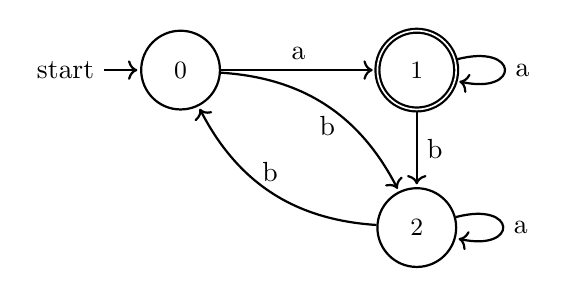
\begin{tikzpicture}[automata]
        % Define the states
        % State 0 is the initial state
        \node[state, initial] (q0) at (0, 0) {0};
        % State 1 is the accepting state, positioned to the top right
        \node[state, accepting] (q1) at (3, 0) {1};
        % State 2 is positioned to the bottom right
        \node[state] (q2) at (3, -2) {2};

        % Define the transitions
        \path[->]
          % Transitions from q0
          (q0) edge [left] node [above] {a} (q1)
               edge [bend left] node [below] {b} (q2)
          % Transitions from q1
          (q1) edge [loop right] node {a} ()
               edge node [right] {b} (q2)
          % Transitions from q2
          (q2) edge [bend left] node [above] {b} (q0)
               edge [loop right] node {a} ();
      \end{tikzpicture}
      \caption{Note that by definition of the transition function, every single state must have exactly one outgoing transition for every symbol in $\Sigma$.} 
      \label{fig:dfa}
    \end{figure}
  \end{definition}

  \begin{definition}[Recognized Language of a DFA]
    Let $w = a_1 a_2 \ldots a_n$ be a string over alphabet $\Sigma$. The DFA $M$ \textbf{accepts} (or computes, or matches) the string $w$ if a sequence of states $r_0, r_1, \ldots, r_n$ exists in $Q$ with the following conditions. 
    \begin{enumerate}
      \item $r_0 = q_0$. 
      \item $r_{i+1} = \delta(r_i, a_{i+1})$ for $i = 0, \ldots, n-1$ 
      \item $r_n \in F$. 
    \end{enumerate}
    The set of all words that are accepted by a DFA $L(M)$ is called the \textbf{language generated by $M$}. 
  \end{definition}

  \begin{definition}[Nondeterministic Finite Automaton]
    A \textbf{nondeterministic finite automaton (NFA)} is a 5-tuple $M = (Q, \Sigma, \delta, q_0, F)$ consisting of 
    \begin{enumerate}
      \item a finite set of states $Q$
      \item a finite set of input symbols called the alphabet $\Sigma$
      \item a transition function $\delta: Q \times (\Sigma \cup \{\epsilon\}) \to 2^Q$\footnote{$2^Q$ denotes the power set of $Q$.}
      \item an initial state $q_0 \in Q$ 
      \item a set of accepting states $F \subset Q$
    \end{enumerate}
    where $\epsilon$ denotes an empty string. There are edges labeled with $\epsilon$, which allows you to traverse to another node at no cost. 

    \begin{figure}[H]
      \centering
      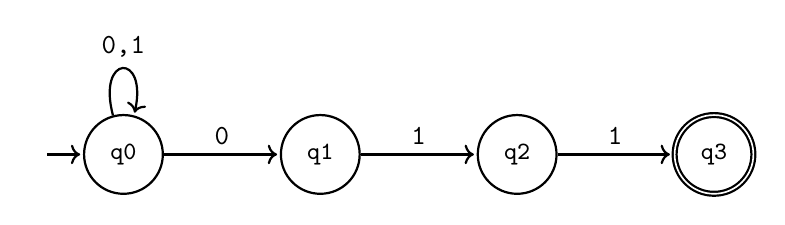
\begin{tikzpicture}[automata, node distance=2.5cm]
        
        % --- States ---
        % Using \texttt for labels as requested
        \node[state, initial, initial text=] (q0) {\texttt{q0}};
        \node[state] (q1) [right=of q0] {\texttt{q1}};
        \node[state] (q2) [right=of q1] {\texttt{q2}};
        \node[state, accepting] (q3) [right=of q2] {\texttt{q3}};

        % --- Transitions ---
        \path
          % Nondeterminism occurs here: on '0', it can loop or go right.
          (q0) edge [loop above] node {\texttt{0,1}} (q0)
          (q0) edge node {\texttt{0}} (q1)
          (q1) edge node {\texttt{1}} (q2)
          (q2) edge node {\texttt{1}} (q3);
          
      \end{tikzpicture}
      \caption{An NFA accepting strings that end in \texttt{011}. Nondeterminism is evident at state \texttt{q0} upon reading a \texttt{0}.}
      \label{fig:nfa_endswith011}
    \end{figure}

    The \textbf{epsilon closure} of a set of nodes is the set plus any other nodes that you can traverse through $\epsilon$-edges. 
  \end{definition} 

  \begin{definition}[Recognized Language of an NFA]
    Let $w = a_1 a_2 \ldots a_n$ be a string over alphabet $\Sigma$. The DFA $M$ \textbf{accepts} (or computes, or matches) the string $w$ if a sequence of states $r_0, r_1, \ldots, r_n$ exists in $Q$ with the following conditions. 
    \begin{enumerate}
      \item $r_0 = q_0$. 
      \item $r_{i+1} \in \delta(r_i, a_{i+1})$ for $i = 0, \ldots, n-1$ 
      \item $r_n \in F$. 
    \end{enumerate}
    The set of all words that are accepted by a DFA $L(M)$ is called the \textbf{language generated by $M$}. 
  \end{definition}

  \begin{algo}[Converting DFA into NFA]
    This may seem obvious, but we need to be slightly careful. 
  \end{algo}

  \begin{definition}[Operations on Finite Automata]
    Let $M_1, M_2$ be two finite automata over the same alphabet $\Sigma$. Then, 
    \begin{enumerate}
      \item \textit{Union}. The union $M_1 \cup M_2$ is defined to be the FA $M$ satisfying $L(M) = L(M_1) \cup L(M_2)$. 
      \item \textit{Complement}. The complement $M_1^c$ is defined to be the FA $M$ satisfying $L(M) = L(M_1)^c \subset \Sigma^\ast$. 
      \item \textit{Intersection}. The intersection $M_1 \cap M_2$ is defined to be the DFA $M$ satisfying $L(M) = L(M_1) \cap L(M_2)$. 
    \end{enumerate}
  \end{definition}

  \begin{lemma}[Union of NFA]
    The union of two NFAs $M_1, M_2$ is simple since you can make a new start node and connect it to the start nodes of the two NFAs with an $\epsilon$-edge. 

    \begin{figure}[H]
      \centering
      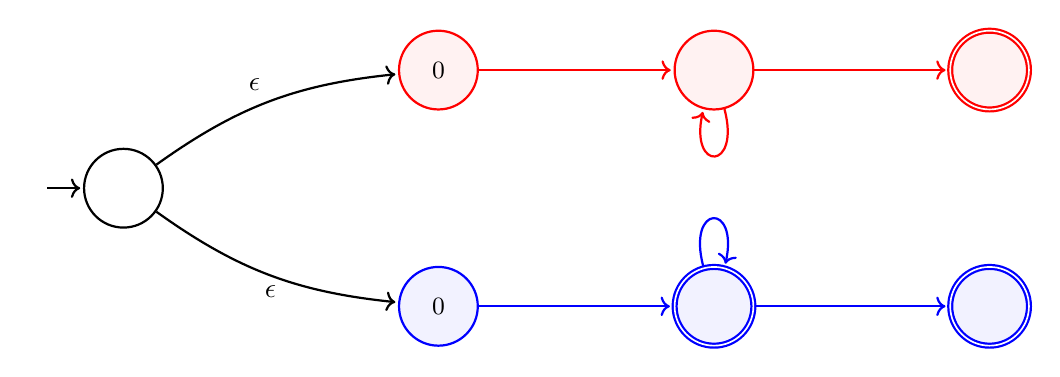
\begin{tikzpicture}[automata]
        % --- NEW BLACK START NODE ---
        \node[state, initial, initial text=] (start) at (-4, 1.5) {};

        % --- RED NFA (Top) ---
        \begin{scope}[every state/.append style={draw=red, fill=red!5}, 
                      every edge/.append style={draw=red}]
          \node[state] (r0) at (0, 3) {0};
          \node[state] (r1) [right=of r0] {};
          \node[state, accepting] (r2) [right=of r1] {};

          \path
            (r0) edge (r1)
            (r1) edge [loop below] (r1)
            (r1) edge (r2);
        \end{scope}

        % --- BLUE NFA (Bottom) ---
        \begin{scope}[every state/.append style={draw=blue, fill=blue!5}, 
                      every edge/.append style={draw=blue}]
          \node[state] (b0) at (0, 0) {0};
          \node[state, accepting] (b1) [right=of b0] {};
          \node[state, accepting] (b2) [right=of b1] {};

          \path
            (b0) edge (b1)
            (b1) edge [loop above] (b1)
            (b1) edge (b2);
        \end{scope}

        % --- CONNECTING EDGES (Black with epsilon labels) ---
        \path
          (start) edge [draw=black, bend left=15] node {$\epsilon$} (r0)
          (start) edge [draw=black, bend right=15] node [below] {$\epsilon$} (b0);
      \end{tikzpicture}
      \caption{Combined NFA with epsilon transitions and a shared start node.}
      \label{fig:nfa_union}
    \end{figure}
  \end{lemma}

  \begin{lemma}[Union of DFA]
    You should convert them to NFAs (which is trivial), then take the union, and then convert them back. 
  \end{lemma}

  \begin{lemma}[Complement of DFA]
    We just flip all the accept and not accept states. 
  \end{lemma}

  However, this doesn't work for an NFA. 

  \begin{example}[Cannot Flip Accept States in NFA]
    \begin{figure}[H]
      \centering
      \begin{subfigure}[b]{0.48\textwidth}
        \centering
        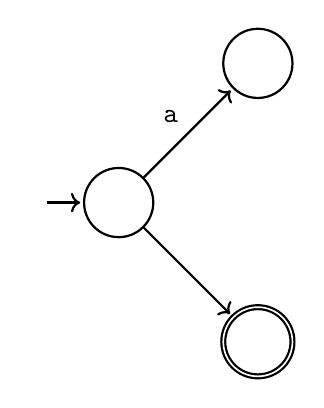
\begin{tikzpicture}[automata, node distance=2.5cm, every state/.style={thick}]
          % Left NFA
          \node[state, initial, initial text=] (q0) {};
          \node[state] (q1) [above right=of q0] {};
          \node[state, accepting] (q2) [below right=of q0] {};

          \path[->]
            (q0) edge node {\texttt{a}} (q1)
            (q0) edge (q2);
        \end{tikzpicture}
        \caption{Accepts \texttt{a}.}
        \label{fig:nfa_left}
      \end{subfigure}
      \hfill 
      \begin{subfigure}[b]{0.48\textwidth}
        \centering
        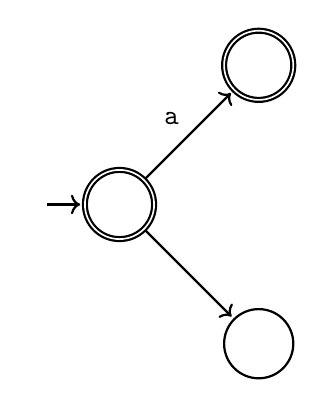
\begin{tikzpicture}[automata, node distance=2.5cm, every state/.style={thick}]
          % Right NFA
          \node[state, initial, accepting, initial text=] (q3) {};
          \node[state, accepting] (q4) [above right=of q3] {};
          \node[state] (q5) [below right=of q3] {};

          \path[->]
            (q3) edge node {\texttt{a}} (q4)
            (q3) edge (q5);
        \end{tikzpicture}
        \caption{Also accepts \texttt{a}, as well as the empty string.}
        \label{fig:nfa_right}
      \end{subfigure}
      \caption{}
      \label{fig:nfa_comparison}
    \end{figure}
  \end{example}

  \begin{lemma}[Complement of NFA]
    Therefore, you must turn an NFA into a DFA and do the complement, and then turn it back. 
  \end{lemma}

  \begin{theorem}[Accepting Nothing]
    We can check if a DFA or NFA accepts nothing by doing BFS and seeing if we can get to an accepting state. 
  \end{theorem}

  \begin{theorem}[Equivalence of NFA/DFAs]
    We can check if two DFAs or two NFAs are equivalent using the rule 
    \begin{equation}
      A = B \iff \overline{A} \cap B \emptyset, A \cap \overline{B} = \emptyset
    \end{equation}
    Therefore, we can check if two regex's are equivalent by converting them into DFAs first. 
  \end{theorem}

  Note that checking equivalence is a very nontrivial thing for algorithms, and in fact is provably impossible to check for arbitrary algorithms (called undecidability). 

  In general, DFAs are known to be the easiest to compute. You can implement this basically as a giant hash table, with the accepting states stored in a list or something. 

  \begin{example}[Computing a DFA]
    Consider the DFA above, and the string \texttt{ababba}. 
  \end{example}

  In general, DFAs are preferred by computers, while humans prefer regular expressions. We want to bridge them somehow so that we can convert regexes to DFAs, and we do this with nondeterministic finite automata. This allows us to write a nice declarative. 

  The problem with NFAs is that it may take an exponential time to compute due to possible branching factors at every node. It turns out that we can turn an NFA into a DFA, which may theoretically have exponentially more nodes, but in general does not. 

  \begin{algo}[Converting NFA to DFA]
    This is basically a fancy BFS algorithm. A DFA state is going to be a set of NFA states. Finally, the accepting state of the NFA is any state that contains the accepting state of the DFA. 
  \end{algo}

  \begin{example}[Converting NFA to DFA]
    \begin{figure}[H]
      \centering
      \begin{subfigure}[b]{0.48\textwidth}
        \centering
        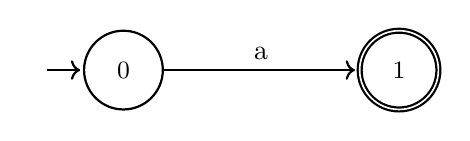
\begin{tikzpicture}[automata]
          % Define the states
          \node[state, initial, initial text=] (q0) {0};
          \node[state, accepting] (q1) [right=of q0] {1};

          % Define the transition
          \path[->]
            (q0) edge node {a} (q1);
        \end{tikzpicture}
        \caption{}
      \end{subfigure}
      \hfill 
      \begin{subfigure}[b]{0.48\textwidth}
        \centering
        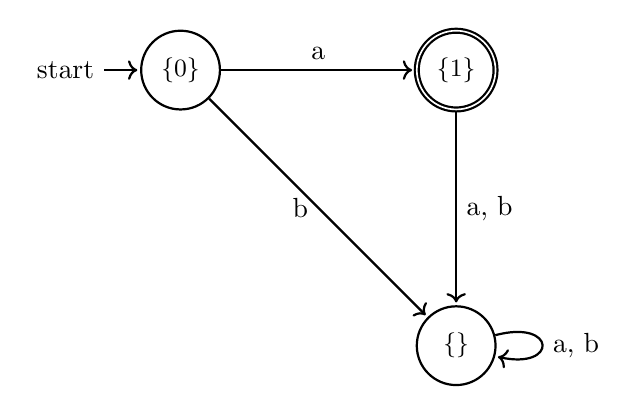
\begin{tikzpicture}[automata]
          % Define the states
          \node[state, initial] (q0) {$\{0\}$};
          \node[state, accepting] (q1) [right=of q0] {$\{1\}$};
          \node[state] (q2) [below=of q1] {$\{\}$}; % Dead state

          % Define the transitions
          \path[->]
            % From state 0
            (q0) edge node {a} (q1)
                 edge node [left] {b} (q2)
            % From state 1 (already accepted 'a', so any further input is a fail)
            (q1) edge node [right] {a, b} (q2)
            % From the dead state (stay here forever)
            (q2) edge [loop right] node [right] {a, b} (q2);
        \end{tikzpicture}
        \caption{}
      \end{subfigure}
      \caption{}
    \end{figure}
  \end{example}

  \begin{example}[Converting NFA to DFA]
    \begin{figure}[H]
      \centering 
      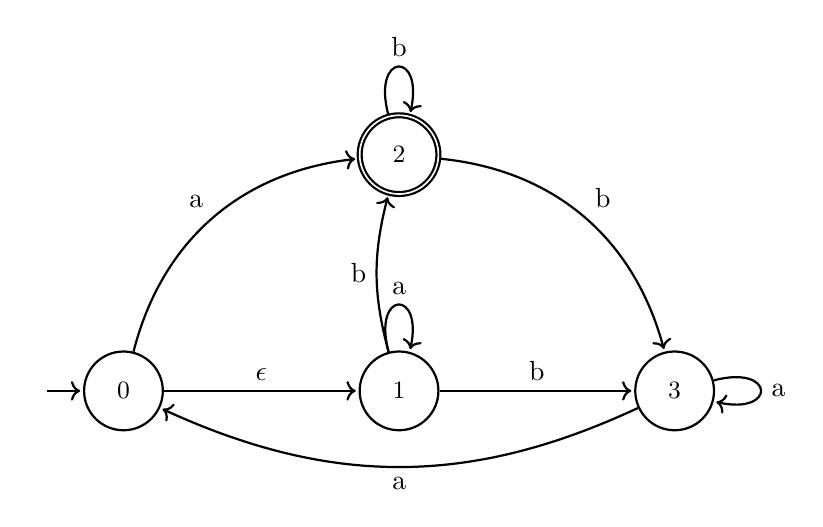
\begin{tikzpicture}[automata]
        % Define the states
        \node[state, initial, initial text=] (q0) at (0, 0) {0};
        \node[state] (q1) at (3.5, 0) {1};
        \node[state, accepting] (q2) at (3.5, 3) {2};
        \node[state] (q3) at (7, 0) {3};

        % Define the transitions
        \path[->]
          % Transitions from state 0
          (q0) edge node {$\epsilon$} (q1)
               edge [bend left=35] node {a} (q2)
          % Transitions from state 1
          (q1) edge [loop above] node {a} ()
               edge [bend left=15] node {b} (q2)
               edge node {b} (q3)
          % Transitions from state 2
          (q2) edge [loop above] node {b} ()
               edge [bend left=35] node {b} (q3)
          % Transitions from state 3
          (q3) edge [loop right] node {a} ()
               edge [bend left=25] node {a} (q0);
      \end{tikzpicture}
      \caption{NFA.} 
      \label{fig:nfa_to_dfa}
    \end{figure}

    \begin{figure}[H]
      \centering 
      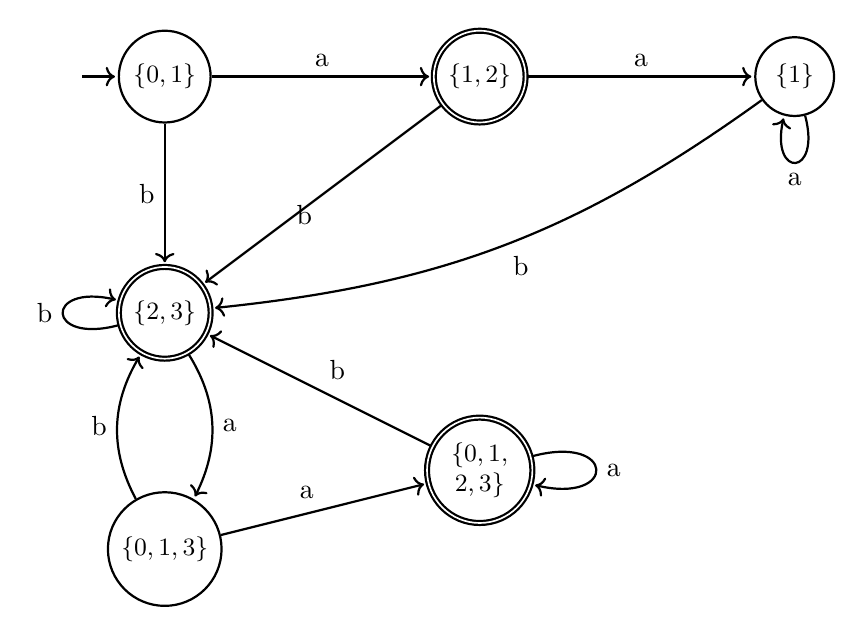
\begin{tikzpicture}[automata]
        % Define the states
        \node[state, initial, initial text=] (s01)   at (0, 4)  {$\{0,1\}$};
        \node[state, accepting] (s12)   at (4, 4)  {$\{1,2\}$};
        \node[state] (s1)    at (8, 4)  {$\{1\}$};
        \node[state, accepting] (s23)   at (0, 1)  {$\{2,3\}$};
        \node[state, accepting] (s0123) at (4, -1) {$\{0,1,$\\$2,3\}$}; 
        \node[state] (s013)  at (0, -2) {$\{0,1,3\}$};

        % Define the transitions
        \path[->]
          (s01) edge node {a} (s12)
                edge node [left] {b} (s23)
          (s12) edge node {a} (s1)
                edge node [below left] {b} (s23)
          (s1)  edge [loop below] node {a} (s1)
                edge [bend left=15] node {b} (s23)
          (s23) edge [loop left] node {b} (s23)
                edge [bend left=30] node {a} (s013)
          (s013) edge [bend left=30] node {b} (s23)
                 edge node {a} (s0123)
          (s0123) edge [loop right] node {a} (s0123)
                  edge node [above right] {b} (s23);
      \end{tikzpicture}
      \caption{DFA.} 
      \label{fig:nfa_to_dfa2}
    \end{figure}
  \end{example}

  \begin{algo}[Converting RegEx to NFA]
    This is a recursive algorithm. 
    \begin{enumerate}
      \item \textit{Symbol}. A symbol $a \in A$ is converted to a simple one edge graph. This is one of the base cases. 

        \begin{figure}[H]
          \centering 
          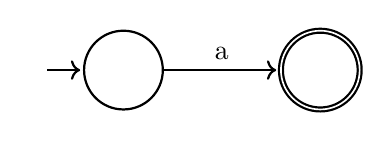
\begin{tikzpicture}[shorten >=1pt, node distance=2.5cm, on grid, auto, thick]
            % Define the states
            \node[state, initial, initial text=] (q0) {};
            \node[state, accepting] (q1) [right=of q0] {};

            % Define the transition
            \path[->]
              (q0) edge node {a} (q1);
          \end{tikzpicture}
          \caption{} 
        \end{figure}

      \item \textit{Epsilon}. The $\epsilon$ is converted to just an accepting state. Note that it can't take in an input. This is another base case. 

        \begin{figure}[H]
          \centering 
          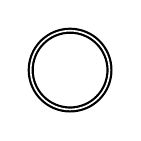
\begin{tikzpicture}[shorten >=1pt, node distance=2.5cm, on grid, auto, thick]
            % Define the states
            \node[state, accepting, initial text=] (q1) {};
          \end{tikzpicture}
          \caption{} 
        \end{figure}

      \item \textit{Or}. Given two NFAs representing $R_1$ and $R_2$, we take the start node and connect it to the start nodes of the two NFAs with an $\epsilon$-edge.\footnote{Note that the presence of $\epsilon$-edges makes things a lot easier for us.}

        \begin{figure}[H]
          \centering
          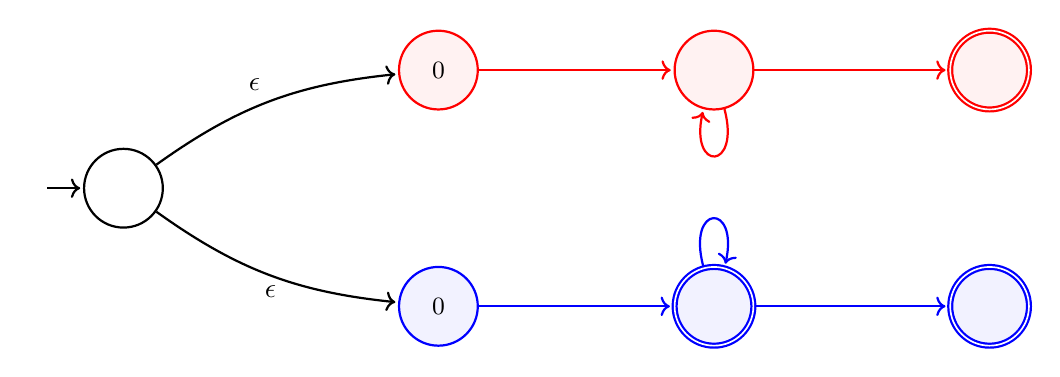
\begin{tikzpicture}[automata]
            % --- NEW BLACK START NODE ---
            \node[state, initial, initial text=] (start) at (-4, 1.5) {};

            % --- RED NFA (Top) ---
            \begin{scope}[every state/.append style={draw=red, fill=red!5}, 
                          every edge/.append style={draw=red}]
              \node[state] (r0) at (0, 3) {0};
              \node[state] (r1) [right=of r0] {};
              \node[state, accepting] (r2) [right=of r1] {};

              \path
                (r0) edge (r1)
                (r1) edge [loop below] (r1)
                (r1) edge (r2);
            \end{scope}

            % --- BLUE NFA (Bottom) ---
            \begin{scope}[every state/.append style={draw=blue, fill=blue!5}, 
                          every edge/.append style={draw=blue}]
              \node[state] (b0) at (0, 0) {0};
              \node[state, accepting] (b1) [right=of b0] {};
              \node[state, accepting] (b2) [right=of b1] {};

              \path
                (b0) edge (b1)
                (b1) edge [loop above] (b1)
                (b1) edge (b2);
            \end{scope}

            % --- CONNECTING EDGES (Black with epsilon labels) ---
            \path
              (start) edge [draw=black, bend left=15] node {$\epsilon$} (r0)
              (start) edge [draw=black, bend right=15] node [below] {$\epsilon$} (b0);
          \end{tikzpicture}
          \caption{Combined NFA with epsilon transitions and a shared start node.}
          \label{fig:combined_nfa_epsilon}
        \end{figure}

      \item \textit{Concatenation}. For $R_1 R_2$, we combine the two NFAs by taking all accepting states in $R_1$ and connect them to the start of $R_2$ with an $\epsilon$-edge. Then, we change the accepting states of $R_1$ to regular states. 

        \begin{figure}[H]
          \centering
          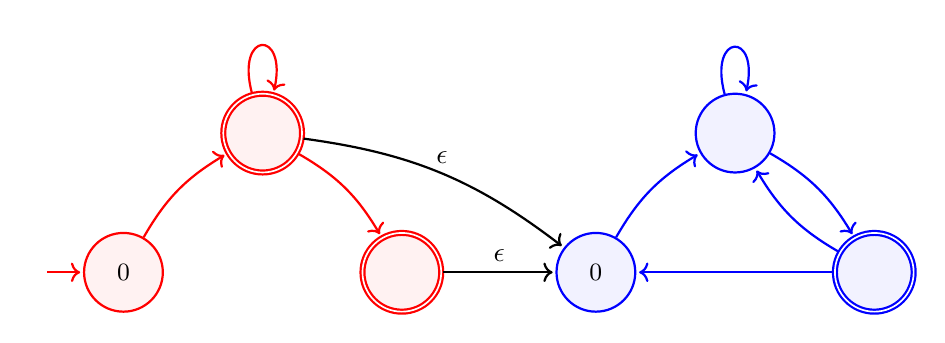
\begin{tikzpicture}[automata, node distance=2.5cm]
            % --- RED NFA (Left) ---
            \begin{scope}[every state/.append style={draw=red, fill=red!5}, 
                          every edge/.append style={draw=red}]
              \node[state, initial, initial text=] (r0) at (0, 0) {0};
              \node[state, accepting] (r1) [above right=of r0] {};
              \node[state, accepting] (r2) [below right=of r1] {};

              \path
                (r0) edge [bend left=15] (r1)
                (r1) edge [loop above] (r1)
                (r1) edge [bend left=15] (r2);
            \end{scope}

            % --- BLUE NFA (Right) ---
            \begin{scope}[every state/.append style={draw=blue, fill=blue!5}, 
                          every edge/.append style={draw=blue}]
              % Shifted right relative to the red graph
              \node[state] (b0) at (6, 0) {0}; 
              \node[state] (b1) [above right=of b0] {};
              \node[state, accepting] (b2) [below right=of b1] {};

              \path
                (b0) edge [bend left=15] (b1)
                (b1) edge [loop above] (b1)
                (b1) edge [bend left=15] (b2)
                (b2) edge [bend left=15] (b1)
                (b2) edge [] (b0);
            \end{scope}

            % --- CONNECTING EDGE ---
            % Connecting red accepting states to blue start state
            \path
              (r2) edge [draw=black] node [above] {$\epsilon$} (b0)
              (r1) edge [draw=black, bend left=15] node [above] {$\epsilon$} (b0);
          \end{tikzpicture}
          \caption{Sequential composition of two NFAs via epsilon transition.}
          \label{fig:sequential_nfa}
        \end{figure}

      \item \textit{Kleene Start}. Given the NFA of a regex $R$ with start node $0$, to find the NFA of $R^\ast$, we do the following. First, make a new start accepting node $s$ and draw an edge $s \xrightarrow{\epsilon} 0$. This makes $0$ not a start node anymore. Finally, for each accepting node $a$ in the NFA of $R$, draw edges $a \xrightarrow{\epsilon} s$. 

        \begin{figure}[H]
          \centering
          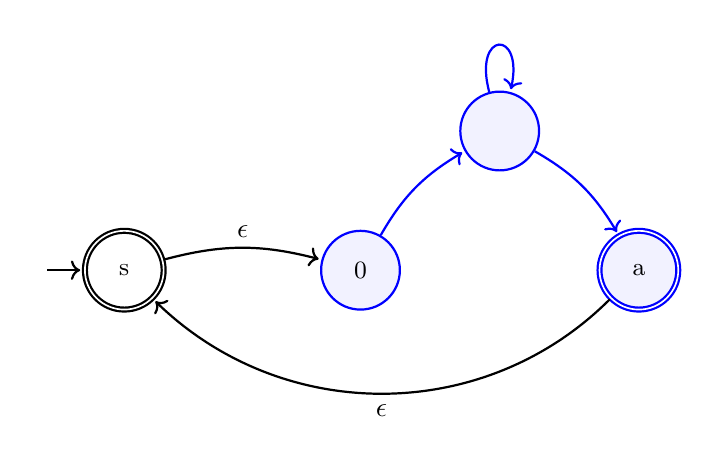
\begin{tikzpicture}[automata, node distance=2.5cm]
            % --- ORIGINAL NFA OF R (Blue) ---
            \begin{scope}[every state/.append style={draw=blue, fill=blue!5}, 
                          every edge/.append style={draw=blue}]
              % The original start node '0' is no longer the entry point
              \node[state] (q0) at (0, 0) {0};
              \node[state] (q1) [above right=of q0] {};
              % Original accepting node 'a'
              \node[state, accepting] (qa) [below right=of q1] {a};

              \path
                (q0) edge [bend left=15] (q1)
                (q1) edge [loop above] (q1)
                (q1) edge [bend left=15] (qa);
            \end{scope}

            % --- NEW KLEENE STAR COMPONENTS (Black) ---
            % 1. New start accepting node 's'
            \node[state, initial, accepting, initial text=] (s) at (-3, 0) {s};

            \path
              % 2. Edge s -> 0
              (s)  edge [draw=black, bend left=15] node [above] {$\epsilon$} (q0)
              % 3. Edge a -> s
              (qa) edge [draw=black, bend left=45] node [below] {$\epsilon$} (s);
          \end{tikzpicture}
          \caption{ The new start node is necessary to avoid the possibility of going around in the NFA and ending at the old start node. }

          \label{fig:kleene_star}
        \end{figure}
        
    \end{enumerate}
  \end{algo}

  So given a regular expression, we convert this to an NFA and then a DFA, which may be (but generally not) exponential complexity with respect to the regex alphabet. But it is independent of the length of the string that we are matching. The matching itself is linear, so we can run millions of bytes-long strings through this DFA. 

  So far, establishing these algorithms to compute DFAs doesn't have an obvious connection to NFAs. It turns out that lexers end up having a bunch of DFAs in them, with different accepting states for different tokens. 

  \begin{example}[NFAs are More Verifiable to Humans]
    Consider the language $L$ of all comments that have delimiters of the form \texttt{/\# ... \#/}. How would we write this as a regular expression? 
    \begin{enumerate}
      \item Our first intuition would be something like \texttt{/\#(.*)\#/}, but this includes strings of form \texttt{/\#\#//\#\#/}, which is two comments. 
      \item We may try to write \texttt{/\#([\^{}\#]|\#[\^{}/])*\#/}, but this includes strings of form \texttt{/\#\#\#/...\#/}, which again isn't viable. 
    \end{enumerate}
    Generally, when you have to keep thinking of edge cases and you`re hacking things, you're on the losing side. However, if we think of this in terms of an NFA, this becomes much better. 

    \begin{figure}[H]
      \centering
      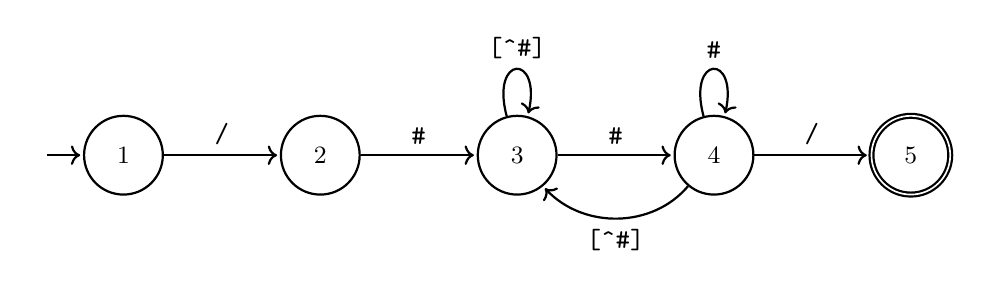
\begin{tikzpicture}[automata, node distance=2.5cm]
        
        % --- States ---
        % Node labels wrapped in \texttt{}
        \node[state, initial, initial text=] (q0) at (0, 0) {1};
        \node[state] (q1) [right=of q0] {2};
        \node[state] (q2) [right=of q1] {3};
        \node[state] (q3) [right=of q2] {4};
        \node[state, accepting] (qa) [right=of q3] {5};

        % --- Edges ---
        % Edge labels wrapped in \texttt{}
        % Note: # still needs escaping as \# inside \texttt{}
        \path
          (q0) edge node {\texttt{/}} (q1)
          (q1) edge node {\texttt{\#}} (q2)
          (q2) edge [loop above] node {\texttt{[\^{}\#]}} (q2)
          (q2) edge node {\texttt{\#}} (q3)
          (q3) edge [loop above] node {\texttt{\#}} (q3)
          (q3) edge node {\texttt{/}} (qa)
          (q3) edge [bend left=50] node [below] {\texttt{[\^{}\#]}} (q2);
          
      \end{tikzpicture}
      \caption{An NFA is much more intuitive to verify.}
      \label{fig:nfa_original_texttt}
    \end{figure}
  \end{example}

  \begin{algo}[NFA to RegEx]
    There are three rules to converting an NFA $M$ with start state $s$ and accepting states $F$ to RegEx's. To do this, we actually put this into an intermediate form called a \textit{generalized NFA}, which has regex's in edge labels, not just symbols. First, add a new start $S$ and connect $S \xrightarrow{\epsilon} s$. Also add a new ``end state'' $E$ and for every $f \in F$, connect $f \xrightarrow{\epsilon} E$. We do this is so that we avoid messy problems where there are multiple edges or loops. 

    \begin{enumerate}
      \item \textit{Eliminate State without Loop}. To delete a node that doesn't have an outgoing edge that loops back to itself, look at all incoming edges and outgoing edges, and directly connect all edges. 

        \begin{figure}[H]
          \centering
          % --- Left Subfigure: Central Node Construction ---
          \begin{subfigure}[b]{0.48\textwidth}
            \centering
            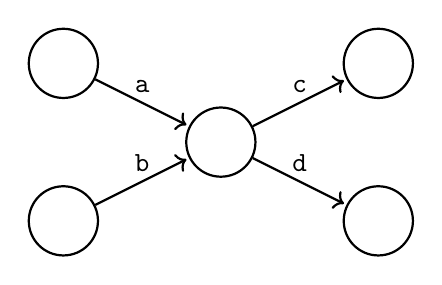
\begin{tikzpicture}[automata, node distance=2.5cm, every state/.style={thick}]
              % Define corners
              \node[state] (q0) at (0, 2) {};
              \node[state] (q1) at (4, 2) {};
              \node[state] (q2) at (0, 0) {};
              \node[state] (q3) at (4, 0) {};
              % Define center
              \node[state] (qc) at (2, 1) {};

              \path[->]
                (q0) edge node [above, pos=0.5] {\texttt{a}} (qc)
                (q2) edge node [above, pos=0.5] {\texttt{b}} (qc)
                (qc) edge node [above, pos=0.5] {\texttt{c}} (q1)
                (qc) edge node [above, pos=0.5] {\texttt{d}} (q3);
            \end{tikzpicture}
            \caption{NFA with intermediate state.}
            \label{fig:nfa_with_center}
          \end{subfigure}
          \hfill 
          % --- Right Subfigure: Direct Connections ---
          \begin{subfigure}[b]{0.48\textwidth}
            \centering
            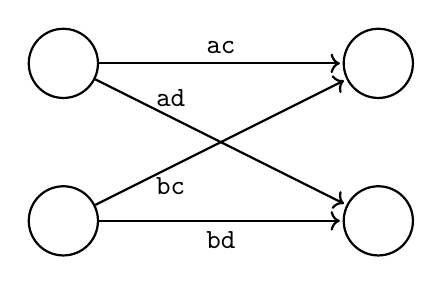
\begin{tikzpicture}[automata, node distance=2.5cm, every state/.style={thick}]
              % Define corners
              \node[state] (q0) at (0, 2) {};
              \node[state] (q1) at (4, 2) {};
              \node[state] (q2) at (0, 0) {};
              \node[state] (q3) at (4, 0) {};

              \path[->]
                (q0) edge node [above] {\texttt{ac}} (q1)
                (q0) edge node [pos=0.3, above] {\texttt{ad}} (q3)
                (q2) edge node [pos=0.3, below] {\texttt{bc}} (q1)
                (q2) edge node [below] {\texttt{bd}} (q3);
            \end{tikzpicture}
            \caption{Direct connections after state removal.}
            \label{fig:nfa_direct}
          \end{subfigure}
          \caption{Comparison of an NFA before and after removing a central state via state elimination.}
          \label{fig:state_elimination_example}
        \end{figure}

      \item \textit{Eliminate State with Loop}. To delete a node that does have an outgoing edge that loops back to itself, 

        \begin{figure}[H]
          \centering
          % --- Left Subfigure: Node with Loop ---
          \begin{subfigure}[b]{0.48\textwidth}
            \centering
            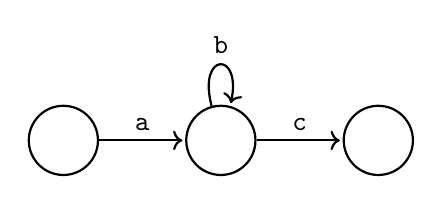
\begin{tikzpicture}[automata, every state/.style={thick}]
              % Defining nodes at specific coordinates
              \node[state] (q0) at (-2, 0) {};
              \node[state] (q1) at (0, 0) {};
              \node[state] (q2) at (2, 0) {};

              \path[->]
                (q0) edge node [above] {\texttt{a}} (q1)
                (q1) edge [loop above] node {\texttt{b}} (q1)
                (q1) edge node [above] {\texttt{c}} (q2);
            \end{tikzpicture}
            \caption{NFA with a self-looping intermediate state.}
            \label{fig:loop_left}
          \end{subfigure}
          \hfill 
          % --- Right Subfigure: Elimination Result ---
          \begin{subfigure}[b]{0.48\textwidth}
            \centering
            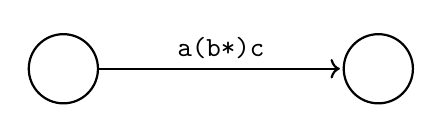
\begin{tikzpicture}[automata, every state/.style={thick}]
              % Middle node removed; outer nodes kept at original coordinates
              \node[state] (q0) at (-2, 0) {};
              \node[state] (q2) at (2, 0) {};

              \path[->]
                (q0) edge node [above] {\texttt{a(b*)c}} (q2);
            \end{tikzpicture}
            \caption{Resulting NFA after eliminating the middle state.}
            \label{fig:loop_right}
          \end{subfigure}
          \caption{Demonstration of the state elimination rule for self-loops.}
          \label{fig:loop_elimination}
        \end{figure}

      \item \textit{Collapse Multiple Edges Between 2 States}. If there are two nodes $n, m$ with multiple edges pointing from $n$ to $m$, then we can just replace it with a single edge that represents an or. 

        \begin{figure}[H]
          \centering
          % --- Left Subfigure: Parallel Edges ---
          \begin{subfigure}[b]{0.48\textwidth}
            \centering
            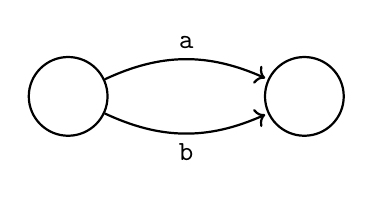
\begin{tikzpicture}[automata]
              \node[state] (q0) at (-1.5, 0) {};
              \node[state] (q1) at (1.5, 0) {};

              \path
                (q0) edge [bend left=25] node [above] {\texttt{a}} (q1)
                (q0) edge [bend right=25] node [below] {\texttt{b}} (q1);
            \end{tikzpicture}
            \caption{Two nodes connected by parallel edges.}
            \label{fig:parallel_left}
          \end{subfigure}
          \hfill 
          % --- Right Subfigure: Combined Edge ---
          \begin{subfigure}[b]{0.48\textwidth}
            \centering
            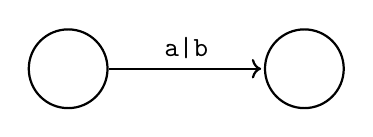
\begin{tikzpicture}[automata]
              \node[state] (q0) at (-1.5, 0) {};
              \node[state] (q1) at (1.5, 0) {};

              \path
                (q0) edge node [above] {\texttt{a|b}} (q1);
            \end{tikzpicture}
            \caption{Parallel edges combined using the union operator.}
            \label{fig:parallel_right}
          \end{subfigure}
          \caption{State elimination rule for combining parallel edges into a single regular expression.}
          \label{fig:elimination_parallel}
        \end{figure}
    \end{enumerate}

    At the end, we will have one edge from $s$ 
  \end{algo}

  \begin{example}[Deriving RegEx for Comments from NFA]
    Let's do the conversion on the NFA above. 
    \begin{enumerate}
      \item \textit{Start}. We add the new start and end states. 

        \begin{figure}[H]
          \centering
          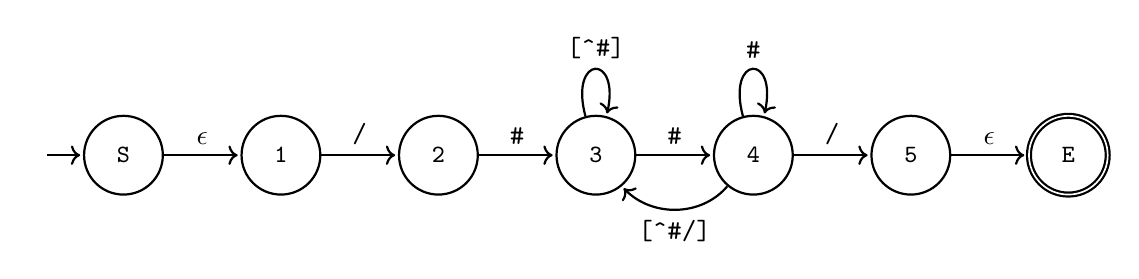
\begin{tikzpicture}[automata, node distance=2cm]
            
            % --- States ---
            \node[state, initial, initial text=] (s) at (-1.5, 0) {\texttt{S}};
            \node[state] (q0) [right=of s] {\texttt{1}};
            \node[state] (q1) [right=of q0] {\texttt{2}};
            \node[state] (q2) [right=of q1] {\texttt{3}};
            \node[state] (q3) [right=of q2] {\texttt{4}};
            \node[state] (q4) [right=of q3] {\texttt{5}};
            \node[state, accepting] (e) [right=of q4] {\texttt{E}};

            % --- Edges ---
            \path
              (s)  edge node {$\epsilon$} (q0)
              (q4) edge node {$\epsilon$} (e)
              (q0) edge node {\texttt{/}} (q1)
              (q1) edge node {\texttt{\#}} (q2)
              (q2) edge [loop above] node {\texttt{[\^{}\#]}} (q2)
              (q2) edge node {\texttt{\#}} (q3)
              (q3) edge [loop above] node {\texttt{\#}} (q3)
              (q3) edge node {\texttt{/}} (q4)
              (q3) edge [bend left=50] node [below] {\texttt{[\^{}\#/]}} (q2);
              
          \end{tikzpicture}
          \caption{Condensed NFA with \texttt{node distance=2cm}.}
        \end{figure}

      \item \textit{State 2}. 

        \begin{figure}[H]
          \centering
          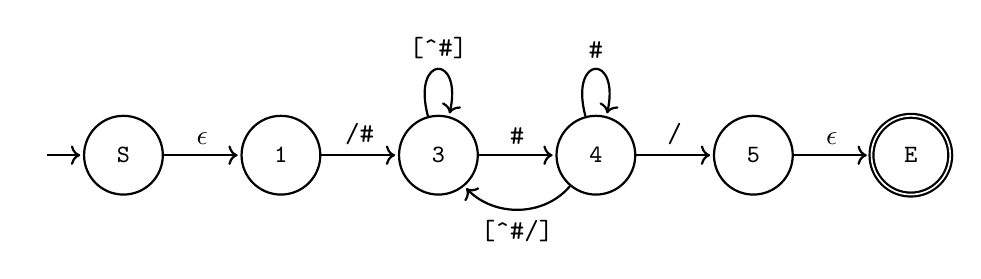
\begin{tikzpicture}[automata, node distance=2cm]
            
            % --- States ---
            \node[state, initial, initial text=] (s) at (-1.5, 0) {\texttt{S}};
            \node[state] (q0) [right=of s] {\texttt{1}};
            \node[state] (q2) [right=of q0] {\texttt{3}};
            \node[state] (q3) [right=of q2] {\texttt{4}};
            \node[state] (q4) [right=of q3] {\texttt{5}};
            \node[state, accepting] (e) [right=of q4] {\texttt{E}};

            % --- Edges ---
            \path
              (s)  edge node {$\epsilon$} (q0)
              (q4) edge node {$\epsilon$} (e)
              (q0) edge node {\texttt{/\#}} (q2)
              (q2) edge [loop above] node {\texttt{[\^{}\#]}} (q2)
              (q2) edge node {\texttt{\#}} (q3)
              (q3) edge [loop above] node {\texttt{\#}} (q3)
              (q3) edge node {\texttt{/}} (q4)
              (q3) edge [bend left=50] node [below] {\texttt{[\^{}\#/]}} (q2);
              
          \end{tikzpicture}
          \caption{Reduced NFA with \texttt{node distance=2cm} and corrected \texttt{\^{}} notation.}
        \end{figure}

      \item \textit{State 1}. 

        \begin{figure}[H]
          \centering
          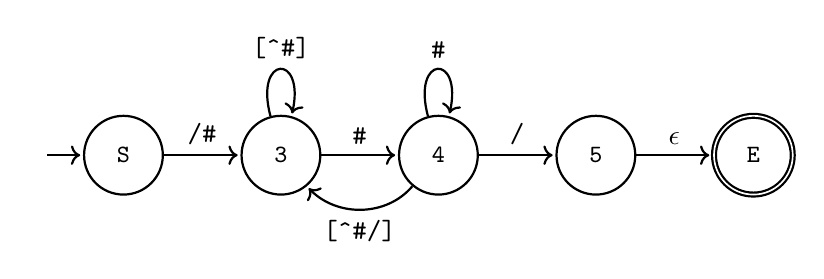
\begin{tikzpicture}[automata, node distance=2cm]
            
            % --- States ---
            \node[state, initial, initial text=] (s) at (-1.5, 0) {\texttt{S}};
            % State 1 has been removed; S now connects directly to State 3
            \node[state] (q2) [right=of s] {\texttt{3}};
            \node[state] (q3) [right=of q2] {\texttt{4}};
            \node[state] (q4) [right=of q3] {\texttt{5}};
            \node[state, accepting] (e) [right=of q4] {\texttt{E}};

            % --- Edges ---
            \path
              % S now goes directly to 3 with the combined label
              (s)  edge node {\texttt{/\#}} (q2)
              (q4) edge node {$\epsilon$} (e)
              % Remaining original transitions
              (q2) edge [loop above] node {\texttt{[\^{}\#]}} (q2)
              (q2) edge node {\texttt{\#}} (q3)
              (q3) edge [loop above] node {\texttt{\#}} (q3)
              (q3) edge node {\texttt{/}} (q4)
              (q3) edge [bend left=50] node [below] {\texttt{[\^{}\#/]}} (q2);
              
          \end{tikzpicture}
          \caption{The NFA after eliminating state \texttt{1}. The transition label \texttt{/\#} is moved to the edge starting from \texttt{S}.}
        \end{figure}

      \item \textit{State 5}. 

        \begin{figure}[H]
          \centering
          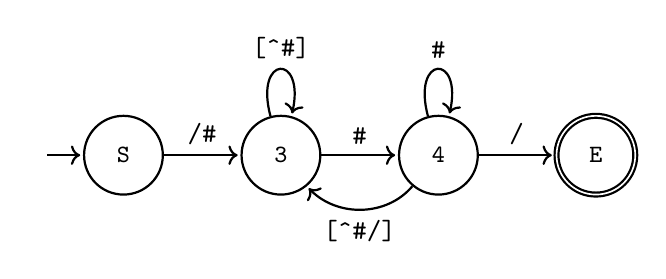
\begin{tikzpicture}[automata, node distance=2cm]
            
            % --- States ---
            \node[state, initial, initial text=] (s) at (-1.5, 0) {\texttt{S}};
            \node[state] (q2) [right=of s] {\texttt{3}};
            \node[state] (q3) [right=of q2] {\texttt{4}};
            % State 5 removed; State 4 now connects directly to E
            \node[state, accepting] (e) [right=of q3] {\texttt{E}};

            % --- Edges ---
            \path
              (s)  edge node {\texttt{/\#}} (q2)
              % q3 (state 4) now goes directly to E with the label '/'
              (q3) edge node {\texttt{/}} (e)
              % Remaining original transitions
              (q2) edge [loop above] node {\texttt{[\^{}\#]}} (q2)
              (q2) edge node {\texttt{\#}} (q3)
              (q3) edge [loop above] node {\texttt{\#}} (q3)
              (q3) edge [bend left=50] node [below] {\texttt{[\^{}\#/]}} (q2);
              
          \end{tikzpicture}
          \caption{The NFA after eliminating state \texttt{5}. The transition to the end state \texttt{E} is now the single character \texttt{/}.}
        \end{figure}

      \item \textit{State 4}. Since state 4 has a loop, we use the second rule. It has an incoming edge from 3 with a \texttt{\#}, a loop edge with a \texttt{\#}, and an outgoing edge to state E with a \texttt{/} and another outgoing edge to state 3 with a \texttt{[\^{}\#]}. Therefore, 
        \begin{align}
          (3 \xrightarrow{\texttt{\#}} 4 \xrightarrow{\texttt{/}} E) & \implies (3 \xrightarrow{\texttt{\#(\#*)/}} E) = (3 \xrightarrow{\texttt{(\#+)/}} E) \\ 
          (3 \xrightarrow{\texttt{\#}} 4 \xrightarrow{\texttt{[\^{}\#]}} 3) & \implies (3 \xrightarrow{\texttt{\#(\#*)[\^{}\#]}} 3) = (3 \xrightarrow{\texttt{(\#+)[\^{}\#]}} 3)
        \end{align}

        \begin{figure}[H]
          \centering
          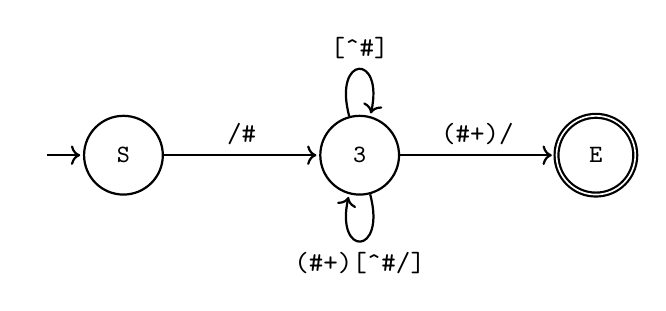
\begin{tikzpicture}[automata, node distance=3cm]
            
            % --- States ---
            \node[state, initial, initial text=] (s) at (-1.5, 0) {\texttt{S}};
            \node[state] (q2) [right=of s] {\texttt{3}};
            \node[state, accepting] (e) [right=of q2] {\texttt{E}};

            % --- Edges ---
            \path
              % Transition from S to 3 remains the same
              (s)  edge node {\texttt{/\#}} (q2)
              
              % Path 3 -> 4 -> E becomes 3 -> #(#*)/ -> E
              (q2) edge node [above] {\texttt{(\#+)/}} (e)
              
              % Path 3 -> 4 -> 3 becomes a new loop on 3: #(#)*[^#]
              % We combine this with the existing loop [^#] using the union operator '|'
              (q2) edge [loop above] node [align=center] {\texttt{[\^{}\#]}} (q2)
              (q2) edge [loop below] node [align=center] {\texttt{(\#+)[\^{}\#/]}} (q2);
              
          \end{tikzpicture}
          \caption{The NFA after eliminating state \texttt{4}. The paths through state 4 are converted into a direct edge to \texttt{E} and an additional loop component on state \texttt{3}.}
        \end{figure}

      \item \textit{State 3}. Since there are two edges that have the same source and destination nodes (both state 3), we should collapse them using rule 3. 

        \begin{figure}[H]
          \centering
          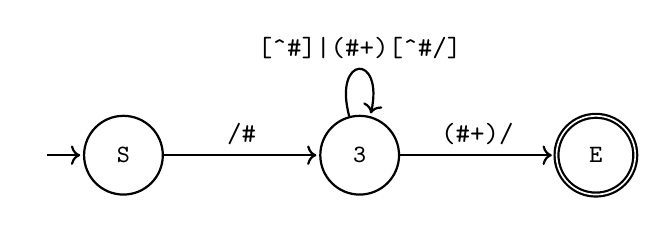
\begin{tikzpicture}[automata, node distance=3cm]
            
            % --- States ---
            \node[state, initial, initial text=] (s) at (-1.5, 0) {\texttt{S}};
            \node[state] (q2) [right=of s] {\texttt{3}};
            \node[state, accepting] (e) [right=of q2] {\texttt{E}};

            % --- Edges ---
            \path
              % Transition from S to 3 remains the same
              (s)  edge node {\texttt{/\#}} (q2)
              
              % Path 3 -> 4 -> E becomes 3 -> #(#*)/ -> E
              (q2) edge node [above] {\texttt{(\#+)/}} (e)
              
              % Path 3 -> 4 -> 3 becomes a new loop on 3: #(#)*[^#]
              % We combine this with the existing loop [^#] using the union operator '|'
              (q2) edge [loop above] node [align=center] {\texttt{[\^{}\#]|(\#+)[\^{}\#/]}} (q2);
          \end{tikzpicture}
          \caption{The NFA after eliminating state \texttt{4}. The paths through state 4 are converted into a direct edge to \texttt{E} and an additional loop component on state \texttt{3}.}
        \end{figure}

      \item \textit{State 3}. Now we can get rid of state 3. 

        \begin{figure}[H]
          \centering
          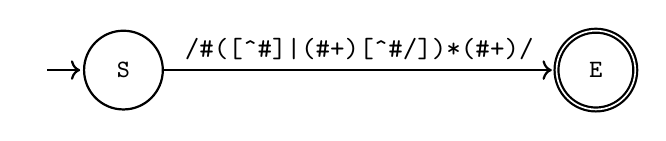
\begin{tikzpicture}[automata, node distance=6cm]
            
            % --- States ---
            % Only the unique start and end states remain
            \node[state, initial, initial text=] (s) at (0, 0) {\texttt{S}};
            \node[state, accepting] (e) [right=of s] {\texttt{E}};

            % --- Edges ---
            % The final regular expression is the concatenation of all eliminated paths
            \path
              (s) edge node [above] {\texttt{/\#([\^{}\#]|(\#+)[\^{}\#/])*(\#+)/}} (e);
              
          \end{tikzpicture}
          \caption{The final NFA after eliminating all intermediate states. The label on the edge represents the final regular expression.}
          \label{fig:final_regex}
        \end{figure}
    \end{enumerate}

    Now we are done. Our regex is 
    \begin{lstlisting}
      /\#([\^{}\#]|(\#+)[\^{}\#/])*(\#+)/ 
    \end{lstlisting}
  \end{example}

\subsection{Tokenizing} 

  Now that we have the tools for lexing, we can finally do it. Really, lexing is just the same thing as tokenizing. 

\section{Parsing} 

\subsection{Context-Free Grammars}

\subsection{Parsing Strategies}

\subsection{Abstract Syntax Trees}

\section{Semantic Analysis} 

\subsection{Symbol Tables} 

\subsection{Type Checking} 

\subsection{Scope Analysis}

\section{Intermediate Representation}

\subsection{IR Design} 

\subsection{Lowering}

\section{Optimization}

\subsection{Local Optimization}

\subsection{Data Flow Analysis}

\subsection{Global Optimization}

\include{sec/backend}
% \section{Jan 7} 

  Will be working in tiger. 
  \begin{enumerate}
    \item \textit{Lexer}. Convert a sequence of characters into a sequence of tokens. Need to talk about DFA, NFA, and regular expressions.  
    \item \textit{Parsing}. Building the abstract syntax tree. e.g. LL parsing (what we are doing) vs LR parsing. MLyac. Trees make everything explicit and so is easier to work with. 
    \item \textit{Type Checking}. 
    \item \textit{IR}. Top of the mountain. 
    \item \textit{Instruction Selection}. 
    \item \textit{Liveness Analysis}. Data flow analysis, which is at the core of a lot of optimization. 
    \item \textit{Register Allocation}. This gives the MIPS assembly, which is text. 
  \end{enumerate}

  Expression evaluates to a value, while a statement is ...
  SMl-NJ, sort of functional.

% \section{Encapsulation}

  % beginning of properties and relationships between classes. 

  \begin{definition}[Encapsulation] 
    % property 
    The result of hiding a representation and implementation in an object. The representation is not visible and cannot be accessed directly from outside the object. Operations are the only way to access and modify an object's representation.  
  \end{definition} 

  public, private, protected + getter/setter methods 
  Python doesn't have (true) encapsulation (or some people say it does, but it lacks access control), since the attributes can be accessed, even when there is name mangling. 


% \section{Inheritance} 

  But so far, these classes are isolated from one another. This is bad because ideally, we want the classes to actually have relationships with each other 

  \begin{definition}[Polymorphism] 
    % property 
    The ability to substitute objects of matching interface for one another at run-time. 
    The idea of \textit{single interface, multiple implementations}. 
  \end{definition}

  \begin{definition}[Toolkit]
    A \textbf{toolkit} is a set of related and reusable classes designed to provide useful, general-purpose functionality. 
  \end{definition}

  \begin{definition}[Framework]
    A \textbf{framework} is a set of cooperating classes that make up a reusable design for a specific class of software. It provides architectural guidance by partitioning the design into abstract classes and defining their responsibilities and collaborations. A developer customizes the framework to a particular application by subclassing and composing instances of framework classes. 
  \end{definition} 

  There are in general two ways: inheritance and object composition. 

  \begin{definition}[Interface Inheritance] 
    \textbf{Interface inheritance} defines a new interface in terms of one or more existing interfaces. 
  \end{definition}

  \begin{definition}[Implementation Inheritance]
    \textbf{Implementation inheritance} defines a new implementation in terms of one or more existing implementations. 
  \end{definition}  

  Class inheritance combines both interface and implementation inheritance, since the subclass.  

  Inheritance is not polymorphism. In inheritance, you get polymorphism when you cast it back to the base class. 

  \href{https://stackoverflow.com/questions/3392352/python-abcs-registering-vs-subclassing}{subclassing vs inheritance}. Invasive vs non-invasive. 
 
  \href{https://peps.python.org/pep-3119/#abcs-vs-duck-typing}{abcs vs duck typing in python (PEP 3119)}.

% \section{Composition} 

  Sometimes, inheritance may not be the right way. There can be a lot of independent properties of a certain class that we would like to model, so we can have child classes across different cross sections. 

  \begin{example}[Visible, Solid, and Movable Objects]
    The example in \href{https://en.wikipedia.org/wiki/Composition_over_inheritance#Example}{Wikipedia} summarizes it nicely. Say you have some an interface to represent any object in the game, and you define three subtypes describing the properties it has. 

    \begin{lstlisting}
      class Object {
      public:
        virtual void update() {}
        virtual void draw() {}
        virtual void collide(Object objects[]) {}
      };

      class Visible : public Object
      {
          Model* model;

      public:
          virtual void draw() override {
              // code to draw a model at the position of this object
          }
      };

      class Solid : public Object
      {
      public:
          virtual void collide(Object objects[]) override {
              // code to check for and react to collisions with other objects
          }
      };

      class Movable : public Object
      {
      public:
          virtual void update() override {
              // code to update the position of this object
          } 
      } 
    \end{lstlisting} 

    If we want to implement the following concrete classes: 
    \begin{enumerate}
      \item class \texttt{Player} which is \texttt{Solid}, \texttt{Movable}, and \texttt{Visible}, 
      \item class \texttt{Cloud}, which is \texttt{Movable} and \texttt{Visible} but not \texttt{Solid}, 
      \item class \texttt{Building} which is \texttt{Solid} and \texttt{Visible} but not \texttt{Movable}, 
      \item class \texttt{Trap} which is \texttt{Solid} but neither \texttt{Visible} not \texttt{Movable}. 
    \end{enumerate} 
    Multiple inheritance is dangerous as we've seen before since it can lead to the diamond problem. One solution to this is the create classes such as \texttt{VisibleAndSolid}, \texttt{VisibleAndMovable}, etc. for all combinations, but this leads to repetitive code. 
  \end{example}

  There must be a better way to organize this, and indeed composition comes to our rescue. The general idea is that rather than modeling the classes with \textit{is-a} relationships, it is better to compose what an object can do with a \textit{has-a} relationship. 

  \begin{definition}[Object Composition]
    \textbf{Object composition} is the principle that objects should contain instances of other classes that implement the desired functionality. 
  \end{definition} 

  \begin{definition}[Delegation]
    
  \end{definition}

  In fact, object composition is so popular that there is a popular saying of \textit{composition over inheritance}. It generally leads to more flexible and modular designs, leveraging the idea of building classes out of \textit{components} rather than trying to find some commonality between them and creating a family tree. 



% \section{Compiling and Linking}

  Now let's talk about how this compiling actually happens. \textit{Compiling} is actually an umbrella term that is misused. Turning at C file into an executable file consists of multiple intermediate steps, one of which is actually compiling, but the whole series is sometimes referred to as compiling. A more accurate term would be \textit{building}. Before we get onto it, there are two types of compilers. 

  \begin{definition}[GCC, CLang]
    The two mainstream compilers used is GCC (with the gdb debugger) and Clang (with lldb). For now, the difference is that 
    \begin{enumerate}
      \item gcc is more established. 
      \item clang is newer and has more features. 
    \end{enumerate}
    A useful flag to know is that we can always specify the name of the (final or intermediary) output file with the \texttt{-o} flag. 
  \end{definition}

  \begin{definition}[Complete Build Process]
    To actually turn a C file into an executable file, we need to go through a series of steps. We start off with the C code, which are the \texttt{.c}, \texttt{.cpp}, or \texttt{.h} files. 
    \begin{enumerate}
      \item \textbf{Preprocessing}: The precompiler step expands the \textit{preprocessor directives} (all the \texttt{\#include} and \texttt{\#define} statements) and removes comments. This results in a \texttt{.i} file. The preprocessor will replace these macros with the actual code. This results in a \texttt{.i} file.
        \begin{lstlisting}
          clang/gcc -E main.c -o main.i
        \end{lstlisting}

      \item \textbf{Compiling}: We take these and generate assembly code. This results in a \texttt{.asm} or \texttt{.s} file.
        \begin{lstlisting}
          clang/gcc -S main.c -o main.s
        \end{lstlisting}

      \item \textbf{Assembler}: We take the assembly code and generate machine code in the form of relocatable binary object code (this is machine code, not assembly). This results in a \texttt{.o} or \texttt{.obj} file.
        \begin{lstlisting}
          clang/gcc -c main.c -o main.o
        \end{lstlisting}

      \item \textbf{Linking}: We take these object files and link them together to form an executable file. This results in a \texttt{.exe} or \texttt{.out} file.
    \end{enumerate}
    The GCC or CLang compiler automates this process for us. For example, \texttt{gcc -c hello.c} generates an object file, taking care of the preprocessing, compiling, and assembling code. Then, \texttt{gcc hello.o} links the object file to generate an executable file. 
  \end{definition}

  There are a lot of questions to be asked here, and we will go through them step by step. 

  \subsection{Precompiling Stage} 

    Just like how Python package managers like conda have specific directories that they find package in, the C library also has a certain directory. 

    \begin{definition}[Standard Library Directory]
      In Linux systems, there are two main directories you look at: 
      \begin{enumerate}
        \item \texttt{/usr/include} contains the standard C library headers.
        \item \texttt{/usr/local/include} contains the headers for libraries that you install yourself.
      \end{enumerate}
      In Mac Silicon, these directories are a little bit more involved. You must first install the xcode command line developer tools, which will then create these directories. 
      \begin{enumerate}
        \item The standard C library headers are in 
          \begin{equation*}
            \texttt{/Library/Developer/CommandLineTools/SDKs/MacOSX*.sdk/usr/include}.
          \end{equation*}
      \end{enumerate}
    \end{definition}

    In here, we can find all the relevant import files like \texttt{stdio.h} and such. When we precompile, the output \texttt{.i} file represents a precompiled C file. It still has C code, but it has been optimized to 
    \begin{enumerate}
      \item Remove comments. 
      \item Replace all the \texttt{\#include} statements with the actual code. 
      \item Replace all the global variables declared in \texttt{\#define} with the actual value.
    \end{enumerate}
    Between x86 and ARM, there are no significant differences in how C files are precompiled. 

    \begin{example}
      Take a look at the following minimal example. 
      \begin{figure}[H]
        \centering 
        \noindent\begin{minipage}{.5\textwidth}
        \begin{lstlisting}[]{Code}
          #include "second.h"
          #define a 3

          int add(int x, int y) {
            return x + y;
          }

          int main() {
            // test comment
            int b = 5; 
            int c = add(a, b);
            int d = subtract(a, b); 
            return 0; 
          }
        \end{lstlisting}
        \end{minipage}
        \hfill
        \begin{minipage}{.49\textwidth}
        \begin{lstlisting}[]{Output}
          int subtract(int a, int b) {
            return a - b; 
          }
          .
          .
          .
          .
          .
          .
          .
          .
          .
          .
          .
        \end{lstlisting}
        \end{minipage}
        \caption{I have included a \texttt{main.c} file that imports statements from a \texttt{second.h} file.} 
        \label{fig:precompile_example}
      \end{figure}
      Now, I run \texttt{gcc -E main.c -o main.i} to generate the precompiled file, which gives me the following. 
      \begin{figure}[H]
        \centering 
        \begin{lstlisting}
          # 1 "main.c"
          # 1 "<built-in>" 1
          # 1 "<built-in>" 3
          # 418 "<built-in>" 3
          # 1 "<command line>" 1
          # 1 "<built-in>" 2
          # 1 "main.c" 2
          # 1 "./second.h" 1
          int subtract(int a, int b) {
            return a - b;
          }
          # 2 "main.c" 2


          int add(int x, int y) {
            return x + y;
          }

          int main() {

            int b = 5;
            int c = add(3, b);
            int d = subtract(3, b);
            return 0;
          }
        \end{lstlisting}
        \caption{The precompiled file. } 
        \label{fig:precompiled_file}
      \end{figure}
      Notice a few things: 
      \begin{enumerate}
        \item The header file \texttt{second.h} has been replaced with the actual code.
        \item The comments have indeed been removed. 
        \item The global variable \texttt{a} has been replaced with the actual value 3. 
      \end{enumerate}
    \end{example}

    This leaves us with the question of what all the rest of the lines that start with a \texttt{\#} are for. They are called \textit{preprocessor directives}.

    \begin{definition}[Preprocessor Directives]
      \textbf{Preprocessor directives} are commands that are executed before the actual compilation begins. These directives allow additional actions to be taken on the C source code before it is compiled into object code. Directives are not part of the C language itself, and they are always prefixed with a \texttt{\#} symbol. 
      \begin{enumerate}
        \item \texttt{\#include} is used to include the contents of a file into the source file. It selects portions of the file to include based on the file name.
        \item \texttt{\#define} is used to define a macro, which is a way to give a name to a constant value or a piece of code. 
        \item \texttt{\#ifdef}, \texttt{\#ifndef}, \texttt{\#else}, and \texttt{\#endif} are used for conditional compilation. 
        \item \texttt{\#error} is used to generate a compilation error. 
        \item \texttt{\#pragma} is used to give the compiler specific instructions. 
      \end{enumerate}
    \end{definition}

  \subsection{Compiling Stage} 

    Once we have precompiled, we can compile the code into assembly code. For the following two examples, we will parse through the general syntax of assembly code. It is quite different between x86 and ARM, so we will use the minimal C code 
    \begin{lstlisting}
      int add(int x, int y) {
        return x + y;
      }

      int main() {
        int a = 3;
        int b = 5; 
        int c = add(a, b);
        return 0; 
      }
    \end{lstlisting}
    for both examples. 

    \begin{example}[x86 Compiled Assembly Language]
      The assmebly code is shown. 
      \begin{lstlisting}[language={[x86masm]Assembler}]
        .
          .file	"main.c"
          .text
          .globl	add
          .type	add, @function
        add:
        .LFB0:
          .cfi_startproc
          endbr64
          pushq	%rbp
          .cfi_def_cfa_offset 16
          .cfi_offset 6, -16
          movq	%rsp, %rbp
          .cfi_def_cfa_register 6
          movl	%edi, -4(%rbp)
          movl	%esi, -8(%rbp)
          movl	-4(%rbp), %edx
          movl	-8(%rbp), %eax
          addl	%edx, %eax
          popq	%rbp
          .cfi_def_cfa 7, 8
          ret
          .cfi_endproc
        .LFE0:
          .size	add, .-add
          .globl	main
          .type	main, @function
        main:
        .LFB1:
          .cfi_startproc
          endbr64
          pushq	%rbp
          .cfi_def_cfa_offset 16
          .cfi_offset 6, -16
          movq	%rsp, %rbp
          .cfi_def_cfa_register 6
          subq	$16, %rsp
          movl	$3, -12(%rbp)
          movl	$5, -8(%rbp)
          movl	-8(%rbp), %edx
          movl	-12(%rbp), %eax
          movl	%edx, %esi
          movl	%eax, %edi
          call	add
          movl	%eax, -4(%rbp)
          movl	$0, %eax
          leave
          .cfi_def_cfa 7, 8
          ret
          .cfi_endproc
        .LFE1:
          .size	main, .-main
          .ident	"GCC: (Ubuntu 9.4.0-1ubuntu1~20.04.2) 9.4.0"
          .section	.note.GNU-stack,"",@progbits
          .section	.note.gnu.property,"a"
          .align 8
          .long	 1f - 0f
          .long	 4f - 1f
          .long	 5
        0:
          .string	 "GNU"
        1:
          .align 8
          .long	 0xc0000002
          .long	 3f - 2f
        2:
          .long	 0x3
        3:
          .align 8
        4:
      \end{lstlisting}
    \end{example}

    \begin{example}[ARM Compiled Assembly Language]
      The assembly code is shown. 
      \begin{lstlisting}[language={[x86masm]Assembler}]
        .
          .section	__TEXT,__text,regular,pure_instructions
          .build_version macos, 14, 0	sdk_version 14, 4
          .globl	_add                            ; -- Begin function add
          .p2align	2
        _add:                                   ; @add
          .cfi_startproc
        ; %bb.0:
          sub	sp, sp, #16
          .cfi_def_cfa_offset 16
          str	w0, [sp, #12]
          str	w1, [sp, #8]
          ldr	w8, [sp, #12]
          ldr	w9, [sp, #8]
          add	w0, w8, w9
          add	sp, sp, #16
          ret
          .cfi_endproc
                                                ; -- End function
          .globl	_main                           ; -- Begin function main
          .p2align	2
        _main:                                  ; @main
          .cfi_startproc
        ; %bb.0:
          sub	sp, sp, #48
          .cfi_def_cfa_offset 48
          stp	x29, x30, [sp, #32]             ; 16-byte Folded Spill
          add	x29, sp, #32
          .cfi_def_cfa w29, 16
          .cfi_offset w30, -8
          .cfi_offset w29, -16
          mov	w8, #0
          str	w8, [sp, #12]                   ; 4-byte Folded Spill
          stur	wzr, [x29, #-4]
          mov	w8, #3
          stur	w8, [x29, #-8]
          mov	w8, #5
          stur	w8, [x29, #-12]
          ldur	w0, [x29, #-8]
          ldur	w1, [x29, #-12]
          bl	_add
          mov	x8, x0
          ldr	w0, [sp, #12]                   ; 4-byte Folded Reload
          str	w8, [sp, #16]
          ldp	x29, x30, [sp, #32]             ; 16-byte Folded Reload
          add	sp, sp, #48
          ret
          .cfi_endproc
                                                ; -- End function
        .subsections_via_symbols
      \end{lstlisting}
    \end{example}
      
    We can see that in both examples, there are generally two types of codes. 
    \begin{enumerate}
      \item The regular CPU operations with registers and memory. 
      \item Some code starts off with some code that starts with a \texttt{.}. Every line that starts with a \texttt{.} are called \textit{assembler directives}. 
    \end{enumerate}
    Let's elaborate more on what these directives are. 

    \begin{definition}[Assembler Directives]
      An \textbf{assembler directives} are instructions in assembly language programming that that give commands to the assembler (which then converts this to an object file) about various aspects of the assembly process, but they do not represent actual CPU instructions that execute in the program. Unlike typical assembly language instructions that directly manipulate registers and execute arithmetic or logical operations, directives are used to organize, control, and provide necessary information for the assembly and linking of binary programs. They can manage memory allocation, define symbols, control compilation settings, and much more. 

      There are general types of directives that are common in both x86 and ARM that we should be aware about: 
      \begin{enumerate}
        \item Section directives. 
        \item Data allocation directives. 
        \item Symbol definition directives. 
        \item Macro and Include directives. 
        \item Debugging and error handling directives. 
      \end{enumerate}
    \end{definition}

    \begin{example}[x86 Assembly Directives]
      Let us elaborate on the specific directives in the x86 assembly code, some of which are in the example above. 
      \begin{enumerate}
        \item \texttt{.file "main.c"} is a directive that tells the assembler that the following code is from the file \texttt{main.c}. It is a form of metadata. 
        \item \texttt{.text} is a directive that tells the assembler that the following code is the text section (the text/code portion of memory) of the program. This is where the actual code is stored. 
        \item \texttt{.globl add} is a directive that tells the assembler that the following code is a global function called \texttt{add}.
        \item \texttt{.type add, @function} is a directive that tells the assembler that the following code is a function.
      \end{enumerate}
    \end{example}

    \begin{example}[ARM Assembly Directives]
      
    \end{example}

    You also see that there are symbols that represent memory addresses. Let's elaborate on what symbols mean. 

    \begin{definition}[Symbol]
      A \textbf{symbol} is a name that is used to refer to a memory location. It can be a function name, a global variable, or a local variable. 
      \begin{enumerate}
        \item Global symbols are symbols that can be referenced by other object files, e.g. non-static functions and global variables. 
        \item Local symbols are symbols that are only visible within the object file, e.g. static functions and local variables. The linker won't know about these types. 
        \item External symbols are referenced by this object file but defined in another object file. 
      \end{enumerate}
    \end{definition}

  \subsection{Objdump} 

    Since we will be using the \texttt{objdump} package quite a lot, it is worth mentioning the different commands you will use and store them here as a reference. For first readers, don't expect to know what each of them do, but rather look back at this for a reference. 

    \subsubsection{ELF and Mach-O Formats}

      Objdump is a command line utility that is used to display information about object files, which are often outputted in a specific format. The two main output file types are called ELF (Executable and Linkable Format) and Mach-O (Mach Object). 

      \begin{definition}[ELF]
        The \textbf{Executable and Linkable Format} (ELF) is a common standard file format for executables, object code, shared libraries, and core dumps. It is analogous to a book, with the following parts: 
        \begin{enumerate}
          \item \textbf{Header}, which is like the cover of the book. It contains metadata about the file, such as the architecture, the entry point, and the sections. 
          \item \textbf{Sections}, which are like chapters. Each section contains the content for some given purpose or use wthin the program. e.g. \texttt{.binary} is just a block of bytes, \texttt{.text} contains the machine code, \texttt{.data} contains initialized data, and \texttt{.bss} contains uninitialized data.
          \item \textbf{Symbol Table}, is like a detailed table of contents of all defined symbols such as functions, external (global) variables, local maps, etc. 
          \item \textbf{Relocation records}, which is like the index of the book that lists references to symbols. 
        \end{enumerate}
        The format is generally as such when you run \texttt{objdump -d -r hello.o} (d represents disassembly and r represents relocation entries).

        \begin{lstlisting}
          ELF header         # file type 

          .text section 
            - code goes here 

          .rodata section
            - read only data 

          .data section 
            - initialized global variables 

          .bss section 
            - uninitialized global variables

          .symtab section 
            - symbol table (symbol name, type, address) 

          .rel.text section 
            - relocation entries for .text section 
            - addresses of instructions that will need to be modified in the executable. 

          .rel.data section 
            - relocation info for .data section 
            - addresses of pointer data that will need to be modified in the merged executable. 

          .debug section 
            - info for symbolic debugging (gcc -g) 
        \end{lstlisting}
      \end{definition}
      
      \begin{definition}[Mach-O]
        
      \end{definition}

    \subsubsection{Objdump Commands}

      \begin{theorem}[File Headers with Objdump]
        Given that you have an object file, the first thing you might want to do is see the file header. You do with this \texttt{objdump -f main.o}. 
        \begin{lstlisting}
          main.o:     file format elf64-x86-64
          architecture: i386:x86-64, flags 0x00000011:
          HAS_RELOC, HAS_SYMS
          start address 0x0000000000000000
        \end{lstlisting}
      \end{theorem}

      \begin{theorem}[Section with Objdump]
        To look at the section headers to get a closer overview, you use \texttt{objdump -h main.o}. 
        \begin{lstlisting}
          main.o:     file format elf64-x86-64

          Sections:
          Idx Name          Size      VMA               LMA               File off  Algn
            0 .text         0000004b  0000000000000000  0000000000000000  00000040  2**0
                            CONTENTS, ALLOC, LOAD, RELOC, READONLY, CODE
            1 .data         00000000  0000000000000000  0000000000000000  0000008b  2**0
                            CONTENTS, ALLOC, LOAD, DATA
            2 .bss          00000000  0000000000000000  0000000000000000  0000008b  2**0
                            ALLOC
            3 .comment      0000002c  0000000000000000  0000000000000000  0000008b  2**0
                            CONTENTS, READONLY
            4 .note.GNU-stack 00000000  0000000000000000  0000000000000000  000000b7  2**0
                            CONTENTS, READONLY
            5 .note.gnu.property 00000020  0000000000000000  0000000000000000  000000b8  2**3
                            CONTENTS, ALLOC, LOAD, READONLY, DATA
            6 .eh_frame     00000058  0000000000000000  0000000000000000  000000d8  2**3
                            CONTENTS, ALLOC, LOAD, RELOC, READONLY, DATA
        \end{lstlisting}
      \end{theorem}

      \begin{theorem}[Disassembly with Objdump]
        Now you might actually want to look at the disassembly of the code, which is what we often use it for. To do this, you use \texttt{objdump -D main.o} to get the entire output. 
        \begin{enumerate}
          \item The leftmost column represents the address of the instruction. 
          \item The next column represents the machine code of the instruction. 
          \item The next column represents the assembly code of the instruction. 
        \end{enumerate}
        \begin{lstlisting}
          main.o:     file format elf64-x86-64

          Disassembly of section .text:

          0000000000000000 <add>:
             0:	f3 0f 1e fa          	endbr64 
             ...
            17:	c3                   	retq   

          0000000000000018 <main>:
            18:	f3 0f 1e fa          	endbr64 
            ...
            4a:	c3                   	retq   

          Disassembly of section .comment:

          0000000000000000 <.comment>:
             0:	00 47 43             	add    %al,0x43(%rdi)
             ...
            2a:	30 00                	xor    %al,(%rax)

          Disassembly of section .note.gnu.property:

          0000000000000000 <.note.gnu.property>:
             0:	04 00                	add    $0x0,%al
            ...

          Disassembly of section .eh_frame:

          0000000000000000 <.eh_frame>:
             0:	14 00                	adc    $0x0,%al
            ...
        \end{lstlisting}
        If you just want to look at the contents of the executable sections, then you can use \texttt{objdump -d main.o}.
        \begin{lstlisting}
          main.o:     file format elf64-x86-64

          Disassembly of section .text:

          0000000000000000 <add>:
             0:	f3 0f 1e fa          	endbr64 
             4:	55                   	push   %rbp
             5:	48 89 e5             	mov    %rsp,%rbp
             8:	89 7d fc             	mov    %edi,-0x4(%rbp)
             b:	89 75 f8             	mov    %esi,-0x8(%rbp)
             e:	8b 55 fc             	mov    -0x4(%rbp),%edx
            11:	8b 45 f8             	mov    -0x8(%rbp),%eax
            14:	01 d0                	add    %edx,%eax
            16:	5d                   	pop    %rbp
            17:	c3                   	retq   

          0000000000000018 <main>:
            18:	f3 0f 1e fa          	endbr64 
            1c:	55                   	push   %rbp
            1d:	48 89 e5             	mov    %rsp,%rbp
            20:	48 83 ec 10          	sub    $0x10,%rsp
            24:	c7 45 f4 03 00 00 00 	movl   $0x3,-0xc(%rbp)
            2b:	c7 45 f8 05 00 00 00 	movl   $0x5,-0x8(%rbp)
            32:	8b 55 f8             	mov    -0x8(%rbp),%edx
            35:	8b 45 f4             	mov    -0xc(%rbp),%eax
            38:	89 d6                	mov    %edx,%esi
            3a:	89 c7                	mov    %eax,%edi
            3c:	e8 00 00 00 00       	callq  41 <main+0x29>
            41:	89 45 fc             	mov    %eax,-0x4(%rbp)
            44:	b8 00 00 00 00       	mov    $0x0,%eax
            49:	c9                   	leaveq 
            4a:	c3                   	retq 
        \end{lstlisting}

        If you want to see the source code intermixed with disassembly, then you can use the \texttt{-S} flag, but make sure that the object file is a generated with debugging information, i.e. use \texttt{gcc -c -g main.c -o main.o}. 
        \begin{figure}[H]
          \centering 
          \begin{lstlisting}
            main.o:     file format elf64-x86-64


            Disassembly of section .text:

            0000000000000000 <add>:
            int add(int x, int y) {
               0:	f3 0f 1e fa          	endbr64 
               4:	55                   	push   %rbp
               5:	48 89 e5             	mov    %rsp,%rbp
               8:	89 7d fc             	mov    %edi,-0x4(%rbp)
               b:	89 75 f8             	mov    %esi,-0x8(%rbp)
              return x + y; 
               e:	8b 55 fc             	mov    -0x4(%rbp),%edx
              11:	8b 45 f8             	mov    -0x8(%rbp),%eax
              14:	01 d0                	add    %edx,%eax
            }
              16:	5d                   	pop    %rbp
              17:	c3                   	retq   

            0000000000000018 <main>:

            int main() {
              18:	f3 0f 1e fa          	endbr64 
              1c:	55                   	push   %rbp
              1d:	48 89 e5             	mov    %rsp,%rbp
              20:	48 83 ec 10          	sub    $0x10,%rsp
              int a = 3; 
              24:	c7 45 f4 03 00 00 00 	movl   $0x3,-0xc(%rbp)
              int b = 5; 
              2b:	c7 45 f8 05 00 00 00 	movl   $0x5,-0x8(%rbp)
              int c = add(a, b); 
              32:	8b 55 f8             	mov    -0x8(%rbp),%edx
              35:	8b 45 f4             	mov    -0xc(%rbp),%eax
              38:	89 d6                	mov    %edx,%esi
              3a:	89 c7                	mov    %eax,%edi
              3c:	e8 00 00 00 00       	callq  41 <main+0x29>
              41:	89 45 fc             	mov    %eax,-0x4(%rbp)
              return 0; 
              44:	b8 00 00 00 00       	mov    $0x0,%eax
            }
              49:	c9                   	leaveq 
              4a:	c3                   	retq  
          \end{lstlisting}
          \caption{Disassembly of the object file back into assembly using \texttt{objdump -d -S main.o}.} 
          \label{fig:disassembly_example_intermixed}
        \end{figure}
        Note that you can always see this disassembly with debuggers like gdb or lldb, but objdump generally works for all architectures. 
      \end{theorem}

      \begin{theorem}[Symbol Table]
        If you want to look at all the symbols existing within the object file, you use \texttt{objdump -t main.o} (t for table of symbols). 
        \begin{enumerate}
          \item The leftmost column represents the address of the symbol. 
          \item The next column represents the type of the symbol. The \texttt{g} and \texttt{l} represent global and local symbols, respectively. The \texttt{O} and \texttt{F} represent object and function symbols, while the \texttt{UND} and \texttt{ABS} represent undefined and absolute symbols. 
          \item The next column represents the section that the symbol is in. 
          \item The next column represents the size of the symbol. 
          \item The last column represents the name of the symbol. 
        \end{enumerate}
        \begin{lstlisting}
          main.o:     file format elf64-x86-64

          SYMBOL TABLE:
          0000000000000000 l    df *ABS*	0000000000000000 main.c
          0000000000000000 l    d  .text	0000000000000000 .text
          0000000000000000 l    d  .data	0000000000000000 .data
          0000000000000000 l    d  .bss	0000000000000000 .bss
          0000000000000000 l    d  .note.GNU-stack	0000000000000000 .note.GNU-stack
          0000000000000000 l    d  .note.gnu.property	0000000000000000 .note.gnu.property
          0000000000000000 l    d  .eh_frame	0000000000000000 .eh_frame
          0000000000000000 l    d  .comment	0000000000000000 .comment
          0000000000000000 g     F .text	0000000000000018 add
          0000000000000018 g     F .text	0000000000000033 main
        \end{lstlisting}
      \end{theorem}

      \begin{theorem}[Relocation Table]
        If you want to look then at the relocation table, then you use \texttt{objdump -r main.o}. 
        \begin{enumerate}
          \item The leftmost column represents the offset of the relocation (i.e. the location within the section where this relocation needs to be applied). 
          \item The second column represents the type of relocation. 
          \item The third column represents the symbol that this relocation references. 
        \end{enumerate}
        \begin{lstlisting}
          main.o:     file format elf64-x86-64

          RELOCATION RECORDS FOR [.text]:
          OFFSET           TYPE              VALUE 
          000000000000003d R_X86_64_PLT32    add-0x0000000000000004


          RELOCATION RECORDS FOR [.eh_frame]:
          OFFSET           TYPE              VALUE 
          0000000000000020 R_X86_64_PC32     .text
          0000000000000040 R_X86_64_PC32     .text+0x0000000000000018
        \end{lstlisting}
      \end{theorem}

  \subsection{Assembling Stage and Object Files}

    Now, once you have gotten the object file, you cannot simply open it up in a text edit as it is in machine code. To actually interpret anything from it, you must \textbf{disassmble} it, meaning that you convert the machine code back into assembly code. The main software that you use to do this is \texttt{objdump}. Let's take a look again at the object file. 

    \begin{figure}[H]
      \centering 
      \begin{lstlisting}
        Disassembly of section .text:

        0000000000000000 <add>:
           0:	f3 0f 1e fa          	endbr64 
           4:	55                   	push   %rbp
           5:	48 89 e5             	mov    %rsp,%rbp
           8:	89 7d fc             	mov    %edi,-0x4(%rbp)
           b:	89 75 f8             	mov    %esi,-0x8(%rbp)
           e:	8b 55 fc             	mov    -0x4(%rbp),%edx
          11:	8b 45 f8             	mov    -0x8(%rbp),%eax
          14:	01 d0                	add    %edx,%eax
          16:	5d                   	pop    %rbp
          17:	c3                   	retq   

        0000000000000018 <main>:
          18:	f3 0f 1e fa          	endbr64 
          1c:	55                   	push   %rbp
          1d:	48 89 e5             	mov    %rsp,%rbp
          20:	48 83 ec 10          	sub    $0x10,%rsp
          24:	c7 45 f4 03 00 00 00 	movl   $0x3,-0xc(%rbp)
          2b:	c7 45 f8 05 00 00 00 	movl   $0x5,-0x8(%rbp)
          32:	8b 55 f8             	mov    -0x8(%rbp),%edx
          35:	8b 45 f4             	mov    -0xc(%rbp),%eax
          38:	89 d6                	mov    %edx,%esi
          3a:	89 c7                	mov    %eax,%edi
          3c:	e8 00 00 00 00       	callq  41 <main+0x29>
          41:	89 45 fc             	mov    %eax,-0x4(%rbp)
          44:	b8 00 00 00 00       	mov    $0x0,%eax
          49:	c9                   	leaveq 
          4a:	c3                   	retq  
      \end{lstlisting}
      \caption{Disassembly of the object file back into assembly using \texttt{objdump -d main.o}. }
      \label{fig:disassembly_example-2}
    \end{figure}

    Let's note a couple things. 
    \begin{enumerate}
      \item The functions are organized by their starting address followed by their name, e.g.  
        \begin{lstlisting}
          0000000000000000 <add>:
        \end{lstlisting}
        Within each function, each line of assembly code is shown. To find the total memory the function takes up, you can just take the address of the last line and subtract it from the address of the first line. Or you can literally count the number of bytes in each line (remember 2 hex is 1 byte). 
      \item The line that calls the \texttt{add} function is \texttt{0x0} (\texttt{00 00 00 00}), with is the \textit{relative target address} intended to be filled in by the linker. The actual assembly line just says that the function continues on to the next line at address \texttt{0x41}. This is because the object file is not aware of where it will be loaded into memory, and all lines with this opcode \texttt{e8 00 00 00 00} is intended to be filled in by the linker. 
      \item Look at address \texttt{0x3c}. It is calling another function, but the values starting from address \texttt{0x3d} is \texttt{00 00 00 00}, which is not the actual address of the function but also a dummy address. This is because the object file is not aware of where the function is located in memory.
    \end{enumerate}

  \subsection{Linking Stage and Relocation}

    \subsubsection{Relocation}

      If the object file is already in machine code, then why do we need a separate linking stage that converts \texttt{main.o} into \texttt{main} the binary? The reason is stated in the previous section: because the object files uses relative memory addressing and does not know about which memory is accessed in other object files, we need to \textbf{relocate} the symbols in the object file to their proper addresses. So how does the linker actually know how to relocate these symbols into their proper addresses? It uses the \textit{relocation table}, which contains information about the addresses that need to be modified in the object file. 

      \begin{figure}[H]
        \centering 
        \begin{lstlisting}
          main.o:     file format elf64-x86-64

          RELOCATION RECORDS FOR [.text]:
          OFFSET           TYPE              VALUE 
          000000000000003d R_X86_64_PLT32    add-0x0000000000000004


          RELOCATION RECORDS FOR [.eh_frame]:
          OFFSET           TYPE              VALUE 
          0000000000000020 R_X86_64_PC32     .text
          0000000000000040 R_X86_64_PC32     .text+0x0000000000000018
        \end{lstlisting}
        \caption{Relocation table for \texttt{main.o} object file. } 
        \label{fig:relocation_table}
      \end{figure}

      Let's talk about how to actually read this table. We can look at the first entry, which shows an offset of \texttt{0x3d}. This represents the offset from the beginning of the \texttt{.text} section where the relocation needs to be applied. Looking back at the disassembly file, this address \texttt{0x3d} is precisely where there was a dummy address \texttt{00 00 00 00}. We want to replace this with the actual address defined in the \texttt{VALUE} column, which is \texttt{add} (with a slight offset of \texttt{0x4}, which is typically used to compensate for the PC-relative addressing mode where the CPU might be adding the length of the instruction to the program counter (PC) before the relocation value is applied). The type of relocation won't be covered in our scope. Let's go through each relocation entry: 

      \begin{enumerate}
        \item The first entry is for the \texttt{add} function. If we look at the disassembly, within the \texttt{main} function, the address \texttt{0x3d} is where the \texttt{add} function is called. The linker will replace the dummy address with the actual address of the \texttt{add} function.
        \begin{lstlisting}
          Disassembly of section .text:

          0000000000000000 <add>:
             0:	f3 0f 1e fa          	endbr64 
             4:	55                   	push   %rbp
             5:	48 89 e5             	mov    %rsp,%rbp
             8:	89 7d fc             	mov    %edi,-0x4(%rbp)
             b:	89 75 f8             	mov    %esi,-0x8(%rbp)
             e:	8b 55 fc             	mov    -0x4(%rbp),%edx
            11:	8b 45 f8             	mov    -0x8(%rbp),%eax
            14:	01 d0                	add    %edx,%eax
            16:	5d                   	pop    %rbp
            17:	c3                   	retq   

          0000000000000018 <main>:
            18:	f3 0f 1e fa          	endbr64 
            1c:	55                   	push   %rbp
            1d:	48 89 e5             	mov    %rsp,%rbp
            20:	48 83 ec 10          	sub    $0x10,%rsp
            24:	c7 45 f4 03 00 00 00 	movl   $0x3,-0xc(%rbp)
            2b:	c7 45 f8 05 00 00 00 	movl   $0x5,-0x8(%rbp)
            32:	8b 55 f8             	mov    -0x8(%rbp),%edx
            35:	8b 45 f4             	mov    -0xc(%rbp),%eax
            38:	89 d6                	mov    %edx,%esi
            3a:	89 c7                	mov    %eax,%edi
            3c:	e8 00 00 00 00       	callq  41 <main+0x29>     <-- here
            41:	89 45 fc             	mov    %eax,-0x4(%rbp)
            44:	b8 00 00 00 00       	mov    $0x0,%eax
            49:	c9                   	leaveq 
            4a:	c3                   	retq  
        \end{lstlisting}
        \item The second and third entries are for the \texttt{.eh\_frame} section. We can see that the offset of \texttt{0x20} and \texttt{0x40} represents the following lines below. They also have dummy addresses that need to be replaced. They are replaced by the address \texttt{.text}, which represents the first address in the \texttt{.text} section, i.e. the address of the \texttt{add} function, and the address \texttt{.text+0x18}, which represents the address of the \texttt{main} function.
        \begin{lstlisting}
          Disassembly of section .eh_frame:

          0000000000000000 <.eh_frame>:
             0:	14 00                	adc    $0x0,%al
             2:	00 00                	add    %al,(%rax)
             4:	00 00                	add    %al,(%rax)
             6:	00 00                	add    %al,(%rax)
             8:	01 7a 52             	add    %edi,0x52(%rdx)
             b:	00 01                	add    %al,(%rcx)
             d:	78 10                	js     1f <.eh_frame+0x1f>
             f:	01 1b                	add    %ebx,(%rbx)
            11:	0c 07                	or     $0x7,%al
            13:	08 90 01 00 00 1c    	or     %dl,0x1c000001(%rax)
            19:	00 00                	add    %al,(%rax)
            1b:	00 1c 00             	add    %bl,(%rax,%rax,1)
            1e:	00 00                	add    %al,(%rax)
            20:	00 00                	add    %al,(%rax)     <-- here for 2nd entry
            22:	00 00                	add    %al,(%rax)
            24:	18 00                	sbb    %al,(%rax)
            26:	00 00                	add    %al,(%rax)
            28:	00 45 0e             	add    %al,0xe(%rbp)
            2b:	10 86 02 43 0d 06    	adc    %al,0x60d4302(%rsi)
            31:	4f 0c 07             	rex.WRXB or $0x7,%al
            34:	08 00                	or     %al,(%rax)
            36:	00 00                	add    %al,(%rax)
            38:	1c 00                	sbb    $0x0,%al
            3a:	00 00                	add    %al,(%rax)
            3c:	3c 00                	cmp    $0x0,%al
            3e:	00 00                	add    %al,(%rax)
            40:	00 00                	add    %al,(%rax)     <-- here for 3rd entry
            42:	00 00                	add    %al,(%rax)
            44:	33 00                	xor    (%rax),%eax
        \end{lstlisting}
      \end{enumerate}
      Therefore, we can see that the object file generates a ``skeleton'' code that contains all the instructions, with some dummy addresses that need to be replaced. The relocation table $T$ tells us exactly where these dummy addresses are in the code and what they need to be replaced with. Therefore, if we want to call a function \texttt{printf} that is in the text section at address \texttt{0x30}, then we can actually look at the value at \texttt{T[30]} to see where the actual address is. At this point, note that we still do not know the actual memory address of \texttt{add}. This is determined by the linker. 

    \subsubsection{Linking with One Object File}

      Now let's see what happens once we link the object file \texttt{main.o} into the final executable \texttt{main}. If we disassemble it, then we can see a few things: 
      \begin{enumerate}
        \item The addresses of all the functions have been changed. \texttt{add} starts on address \texttt{0x1129} rather than \texttt{0x0} and \texttt{main} starts on address \texttt{0x1141} rather than \texttt{0x18}. 
        \item The dummy address \texttt{0x0} of the call to function \texttt{add} in \texttt{main} have been replaced with the actual addresses \texttt{0x1129}. 
      \end{enumerate}

      \begin{lstlisting}
        0000000000001129 <add>:
          1129:	f3 0f 1e fa          	endbr64 
          112d:	55                   	push   %rbp
          112e:	48 89 e5             	mov    %rsp,%rbp
          1131:	89 7d fc             	mov    %edi,-0x4(%rbp)
          1134:	89 75 f8             	mov    %esi,-0x8(%rbp)
          1137:	8b 55 fc             	mov    -0x4(%rbp),%edx
          113a:	8b 45 f8             	mov    -0x8(%rbp),%eax
          113d:	01 d0                	add    %edx,%eax
          113f:	5d                   	pop    %rbp
          1140:	c3                   	retq   

        0000000000001141 <main>:
          1141:	f3 0f 1e fa          	endbr64 
          1145:	55                   	push   %rbp
          1146:	48 89 e5             	mov    %rsp,%rbp
          1149:	48 83 ec 10          	sub    $0x10,%rsp
          114d:	c7 45 f4 03 00 00 00 	movl   $0x3,-0xc(%rbp)
          1154:	c7 45 f8 05 00 00 00 	movl   $0x5,-0x8(%rbp)
          115b:	8b 55 f8             	mov    -0x8(%rbp),%edx
          115e:	8b 45 f4             	mov    -0xc(%rbp),%eax
          1161:	89 d6                	mov    %edx,%esi
          1163:	89 c7                	mov    %eax,%edi
          1165:	e8 bf ff ff ff       	callq  1129 <add>     <-- replaced with actual address
          116a:	89 45 fc             	mov    %eax,-0x4(%rbp)
          116d:	b8 00 00 00 00       	mov    $0x0,%eax
          1172:	c9                   	leaveq 
          1173:	c3                   	retq   
          1174:	66 2e 0f 1f 84 00 00 	nopw   %cs:0x0(%rax,%rax,1)
          117b:	00 00 00 
          117e:	66 90                	xchg   %ax,%ax 
      \end{lstlisting}

    \subsubsection{Global vs External Symbols}

      So far, we have talked about using the \texttt{\#include} as a precompiling command that says ``put all the text from this other file right here.'' Take the following code for instance. 

      \begin{figure}[H]
        \centering 
        \noindent\begin{minipage}{.5\textwidth}
        \begin{lstlisting}[]{Code}
          // file1.c 
          #include "sum.h" 

          int array[2] = {1, 2}; 

          int main() {
            int val = sum(array, 2); 
            return val; 
          }
        \end{lstlisting}
        \end{minipage}
        \hfill
        \begin{minipage}{.49\textwidth}
        \begin{lstlisting}[]{Output}
          // sum.h 
          int sum(int *a, int n) {
            int i, s = 0; 
            for (i = 0; i < n; i++) {
              s += a[i]; 
            }
            return s; 
          }
          .
        \end{lstlisting}
        \end{minipage}
        \caption{Including a header file in \texttt{file1.c} to import functions and variables.}
        \label{fig:include_example}
      \end{figure}

      However, there is another way to do this. We can use \textit{external symbols} to access. Rather than simply copying and pasting the code into the file, the \texttt{extern} keyword marks that the variable or function exists externally to this source file and does not allocate storage for it. 

      \begin{figure}[H]
        \centering 
        \noindent\begin{minipage}{.50\textwidth}
        \begin{lstlisting}[]{Code}
          // main.c
          extern int sum(int *array, int n); 

          int array[2] = {1, 2};

          int main(void) {
            int val = sum(array, 2); 
            return val; 
          }
        \end{lstlisting}
        \end{minipage}
        \hfill
        \begin{minipage}{.49\textwidth}
        \begin{lstlisting}[]{Output}
          // sum.c
          int sum(int *array, int n) {
            int i, s = 0 ; 
            for (int i = 0; i < n; i++) {
                s += array[i];
              }
            return s;
          }
          .
        \end{lstlisting}
        \end{minipage}
        \caption{Using external symbols to access functions and variables.} 
        \label{fig:external_symbols_example}
      \end{figure}
      
      One is not a replacement for the other, so what advantage does this have? Well, as we will see, if we have multiple object (source) files, say \texttt{A.c}, \texttt{B.c}, and \texttt{C.c}, that need to reference the same function or variable \texttt{var} in \texttt{ext.c}, then how would we do this? If we simply put \texttt{\#include "ext.h"} in all the files, then we would have multiple copies of the same code. This means that for each source there would be its own copy of \texttt{var} created and the linker would be unable to resolve this symbol. However, if we put \texttt{extern int var; } at the top of each source file, then only one copy of \texttt{var} would be created (in \texttt{ext.c}), which creates a single instance of \texttt{var} for the linker to resolve. \footnote{https://stackoverflow.com/questions/1330114/whats-the-difference-between-using-extern-and-including-header-files}

      Therefore, there are three types of symbols (variables, functions, etc.) that we need to consider: 
      \begin{enumerate}
        \item \textbf{Global symbols} that are defined in the global scope of a C file. 
        \item \textbf{Local symbols} that are defined in the local scope of a C file, e.g. within functions, loops, etc. 
        \item \textbf{External symbols} that are defined in another C file referenced by the \texttt{extern} keyword.
      \end{enumerate}
      Linkers will only know about global and external symbols, and will have no idea that any local symbols exist. With the information of these two types of symbols and the relocation tables of each object file, the linker can then resolve the addresses of all the symbols in the final binary. 

      The two types of symbols that the linker will know about are the global and external symbols. We can see that external symbols can be problematic if the object files don't know about each other. 

      \begin{example}[Global and Local Symbols]
        Consider the following code where the left file includes the right file. 

        \noindent\begin{minipage}{.5\textwidth}
        \begin{lstlisting}[]{Code}
          // main.c 
          #include "sum.h" 

          int array[2] = {1, 2}; 

          int main() {
            int val = sum(array, 2); 
            return val; 
          }
        \end{lstlisting}
        \end{minipage}
        \hfill
        \begin{minipage}{.49\textwidth}
        \begin{lstlisting}[]{Output}
          // sum.h 
          int sum(int *a, int n) {
            int i, s = 0; 
            for (i = 0; i < n; i++) {
              s += a[i]; 
            }
            return s; 
          }
          .
        \end{lstlisting}
        \end{minipage}
        In the left file, 
        \begin{enumerate}
          \item We define the global symbol \texttt{main()}. 
          \item Inside main, \texttt{val} is a local symbol so the linker knows nothing about it. 
          \item The \texttt{sum} function is an external symbol, and it references a global symbol that's defined in \texttt{sum} the right file. 
          \item The \texttt{array} is a global symbol that is defined in the right file. 
        \end{enumerate}
        In the right file, the linker knows nothing of the local symbols \texttt{i} or \texttt{s}. 
      \end{example}

    \subsubsection{Linking with Multiple Object Files}

      We have seen the case of linking when we simply have one object file. The relocation was simple since the \texttt{.text} section is contiguous and so we needed simple translations of addresses to relocate \texttt{add} and \texttt{main}, along with whatever other sections and files. Now let's consider the case where we have multiple object files.

      \noindent\begin{minipage}{.50\textwidth}
      \begin{lstlisting}[]{Code}
        // main.c
        extern int sum(int *array, int n); 

        int array[2] = {1, 2};

        int main(void) {
          int val = sum(array, 2); 
          return val; 
        }
      \end{lstlisting}
      \end{minipage}
      \hfill
      \begin{minipage}{.49\textwidth}
      \begin{lstlisting}[]{Output}
        // sum.c
        int sum(int *array, int n) {
          int i, s = 0 ; 
          for (int i = 0; i < n; i++) {
              s += array[i];
            }
          return s;
        }
        .
      \end{lstlisting}
      \end{minipage}

      Now they have their own object files shown below, where I also put the source code lines to make it easier to parse. Note that again, in \texttt{main.o} the call to function \texttt{sum} is a dummy address that needs to be replaced. Furthermore, in both \texttt{main.o} and \texttt{sum.o}, the \texttt{.text} section is at address \texttt{0x0}, where the addresses of the function \texttt{main} and \texttt{sum} are, respectively. This causes an overload in the address space. 

      To demonstrate what happens, we look at how the disassembly, symbol tables, and relocation tables are updated before (with the object files) and after (in the binary) linking.  

      \begin{example}[Disassembly of Object Files]
        In here, note that both the \texttt{array} and \texttt{sum} are not initialized and are therefore set to dummy addresses. 
        \begin{lstlisting}
          main.o:     file format elf64-x86-64
          Disassembly of section .text:

          0000000000000000 <main>:
          extern int sum(int *array, int n); 

          int array[2] = {1, 2}; 

          int main(void) {
             0:	f3 0f 1e fa          	endbr64 
             4:	55                   	push   %rbp
             5:	48 89 e5             	mov    %rsp,%rbp
             8:	48 83 ec 10          	sub    $0x10,%rsp
            int val = sum(array, 2); 
             c:	be 02 00 00 00       	mov    $0x2,%esi
            11:	48 8d 3d 00 00 00 00 	lea    0x0(%rip),%rdi        # 18 <main+0x18>  <-- dummy address
            18:	e8 00 00 00 00       	callq  1d <main+0x1d>                          <-- dummy address
            1d:	89 45 fc             	mov    %eax,-0x4(%rbp)
            return val; 
            20:	8b 45 fc             	mov    -0x4(%rbp),%eax
          }
            23:	c9                   	leaveq 
            24:	c3                   	retq  
        \end{lstlisting}
        \begin{lstlisting}
          sum.o:     file format elf64-x86-64
          Disassembly of section .text:

          0000000000000000 <sum>:
          int sum(int *array, int n) {
             0:	f3 0f 1e fa          	endbr64 
             4:	55                   	push   %rbp
             5:	48 89 e5             	mov    %rsp,%rbp
             8:	48 89 7d e8          	mov    %rdi,-0x18(%rbp)
             c:	89 75 e4             	mov    %esi,-0x1c(%rbp)
            int i, s = 0; 
             f:	c7 45 f8 00 00 00 00 	movl   $0x0,-0x8(%rbp)
            for (int i = 0; i < n; i++) {
            16:	c7 45 fc 00 00 00 00 	movl   $0x0,-0x4(%rbp)
            1d:	eb 1d                	jmp    3c <sum+0x3c>
              s += array[i]; 
            1f:	8b 45 fc             	mov    -0x4(%rbp),%eax
            22:	48 98                	cltq   
            24:	48 8d 14 85 00 00 00 	lea    0x0(,%rax,4),%rdx
            2b:	00 
            2c:	48 8b 45 e8          	mov    -0x18(%rbp),%rax
            30:	48 01 d0             	add    %rdx,%rax
            33:	8b 00                	mov    (%rax),%eax
            35:	01 45 f8             	add    %eax,-0x8(%rbp)
            for (int i = 0; i < n; i++) {
            38:	83 45 fc 01          	addl   $0x1,-0x4(%rbp)
            3c:	8b 45 fc             	mov    -0x4(%rbp),%eax
            3f:	3b 45 e4             	cmp    -0x1c(%rbp),%eax
            42:	7c db                	jl     1f <sum+0x1f>
            }
            return s; 
            44:	8b 45 f8             	mov    -0x8(%rbp),%eax
          }
            47:	5d                   	pop    %rbp
            48:	c3                   	retq  
        \end{lstlisting}
        \begin{enumerate}
          \item In \texttt{main.o} at address \texttt{0x0}, we have the \texttt{main} function and this is because everything is stored relatively to the start of main. Once we have linked, \texttt{main} shows the absolute addresses of all the instructions. 
          \item In instruction 11 in \texttt{main.o} we can see that \texttt{48 8d 3d} is the \texttt{lea} instruction, which is the same as that in \texttt{main}. However, the address that is was acting on is \texttt{0x0} since the array has not been initialized yet. We can see in \texttt{main} that the address is now \texttt{0x00002ecf}. 
          \item The comment in \texttt{main} indicates that the final relocated address used to access the \texttt{array} is \texttt{0x4010}. To see relocated addresses in general, just look for the comments and shift them accordingly. 
        \end{enumerate}
        \begin{lstlisting}
          main:     file format elf64-x86-64

          0000000000001129 <main>:
              1129:	f3 0f 1e fa          	endbr64 
              112d:	55                   	push   %rbp
              112e:	48 89 e5             	mov    %rsp,%rbp
              1131:	48 83 ec 10          	sub    $0x10,%rsp
              1135:	be 02 00 00 00       	mov    $0x2,%esi
              113a:	48 8d 3d cf 2e 00 00 	lea    0x2ecf(%rip),%rdi        # 4010 <array>
              1141:	e8 08 00 00 00       	callq  114e <sum>
              1146:	89 45 fc             	mov    %eax,-0x4(%rbp)
              1149:	8b 45 fc             	mov    -0x4(%rbp),%eax
              114c:	c9                   	leaveq 
              114d:	c3                   	retq   

          000000000000114e <sum>:
              114e:	f3 0f 1e fa          	endbr64 
              1152:	55                   	push   %rbp
              1153:	48 89 e5             	mov    %rsp,%rbp
              1156:	48 89 7d e8          	mov    %rdi,-0x18(%rbp)
              115a:	89 75 e4             	mov    %esi,-0x1c(%rbp) 
              ...
        \end{lstlisting}
      \end{example}

      \begin{example}[Symbol Tables of Object Files]
        Let's take a look at the symbol table of each file as well. Again, all of the addresses of each symbol are 0s since they are using relative addressing. The \texttt{array} and \texttt{main} are global symbols since they reside in the global scope, while the \texttt{sum} function is an external and undefined symbol.
        \begin{lstlisting}
          main.o:     file format elf64-x86-64

          SYMBOL TABLE:
          0000000000000000 l    df *ABS*	0000000000000000 main.c
          0000000000000000 l    d  .text	0000000000000000 .text
          0000000000000000 l    d  .data	0000000000000000 .data
          0000000000000000 l    d  .bss	0000000000000000 .bss
          0000000000000000 l    d  .note.GNU-stack	0000000000000000 .note.GNU-stack
          0000000000000000 l    d  .note.gnu.property	0000000000000000 .note.gnu.property
          0000000000000000 l    d  .eh_frame	0000000000000000 .eh_frame
          0000000000000000 l    d  .comment	0000000000000000 .comment
          0000000000000000 g     O .data	0000000000000008 array
          0000000000000000 g     F .text	0000000000000025 main
          0000000000000000         *UND*	0000000000000000 _GLOBAL_OFFSET_TABLE_
          0000000000000000         *UND*	0000000000000000 sum
        \end{lstlisting}
        \begin{lstlisting}
          sum.o:     file format elf64-x86-64

          SYMBOL TABLE:
          0000000000000000 l    df *ABS*	0000000000000000 sum.c
          0000000000000000 l    d  .text	0000000000000000 .text
          0000000000000000 l    d  .data	0000000000000000 .data
          0000000000000000 l    d  .bss	0000000000000000 .bss
          0000000000000000 l    d  .note.GNU-stack	0000000000000000 .note.GNU-stack
          0000000000000000 l    d  .note.gnu.property	0000000000000000 .note.gnu.property
          0000000000000000 l    d  .eh_frame	0000000000000000 .eh_frame
          0000000000000000 l    d  .comment	0000000000000000 .comment
          0000000000000000 g     F .text	0000000000000049 sum
        \end{lstlisting}
        When we have the linked binary, note a few things. 
        \begin{enumerate}
          \item In \texttt{main.o}, the numbers on the left represents the address of the symbol (all 0s since we haven't linked yet and their final addresses aren't known), while the addresses in \texttt{a.out} are all known. 
          \item In \texttt{main.o}, the \texttt{sum} function is an external symbol and is undefined. The linker will need to know where this is. In \texttt{main}, note that the \texttt{sum} function is now a global symbol and is defined, along with the size. We can now see that all the final addresses of each symbol is known, along with their sizes, and the \texttt{UND} marker is now gone as well. 
          \item Only the size of the global variable is known in \texttt{main.o} since we have defined it within the code. However, in \texttt{main}, the linker has now assigned an address to it.
          \item To see the size in bytes of the array, you can look at the address and how much size it takes up. 
        \end{enumerate}
        \begin{lstlisting}
          main:     file format elf64-x86-64

          SYMBOL TABLE:
          ...
          0000000000004008 g     O .data	  0000000000000000              .hidden __dso_handle
          000000000000114e g     F .text	  0000000000000049              sum
          0000000000002000 g     O .rodata	  0000000000000004              _IO_stdin_used
          00000000000011a0 g     F .text	  0000000000000065              __libc_csu_init
          0000000000004020 g       .bss	     0000000000000000              _end
          0000000000001040 g     F .text	  000000000000002f              _start
          0000000000004018 g       .bss	     0000000000000000              __bss_start
          0000000000001129 g     F .text	  0000000000000025              main
          0000000000004018 g     O .data	  0000000000000000              .hidden __TMC_END__
          ...
        \end{lstlisting}
      \end{example}

      \begin{example}[Relocation Tables]
        Ignoring the \texttt{.eh\_frame}, in \texttt{main.o} the relocation table contains entries for \texttt{array} and \texttt{sum} that must be relocated. 
        \begin{lstlisting}
          main.o:     file format elf64-x86-64

          RELOCATION RECORDS FOR [.text]:
          OFFSET           TYPE              VALUE 
          0000000000000014 R_X86_64_PC32     array-0x0000000000000004
          0000000000000019 R_X86_64_PLT32    sum-0x0000000000000004

          RELOCATION RECORDS FOR [.eh_frame]:
          OFFSET           TYPE              VALUE 
          0000000000000020 R_X86_64_PC32     .text 
        \end{lstlisting}
        \begin{lstlisting}
          sum.o:     file format elf64-x86-64

          RELOCATION RECORDS FOR [.eh_frame]:
          OFFSET           TYPE              VALUE 
          0000000000000020 R_X86_64_PC32     .text
        \end{lstlisting}
        We can see a couple things. Namely, there is nothing to be relocated in \texttt{a.out} since everything has been relocated already by the linker. So let's focus on the relocation for \texttt{main.o}. In here, we can see that in the \texttt{.text} section, there are two things being relocated: 
        \begin{enumerate}
          \item The reference to the global variable \texttt{array} is being relocated. In this object file, we look at the offset \texttt{0x14} from the beginning of the \texttt{.text} section, which contains the instruction that needs to access \texttt{array}. This relocation record tells the linker to calculate the 32-bit offset from the instruction (at offset \texttt{0x14}) to the start of \texttt{array}, then adjust it by subtracting 4 bytes. 

          \item The reference to the \texttt{sum} function is being relocated. In this object file, we look at the offset \texttt{0x19} from the beginning of the \texttt{.text} section, which contains the instruction that needs to access \texttt{sum}. This relocation record tells the linker to calculate the 32-bit offset from the instruction (at offset \texttt{0x19}) to the start of the \texttt{.plt} section, then adjust it by subtracting 4 bytes.
        \end{enumerate}
        \begin{lstlisting}
          main:     file format elf64-x86-64 
        \end{lstlisting}
      \end{example}
       
  \subsection{Compiler Optimization}

    We have learned the complete process of compilers, but compilers can be a little smarter than just translating code line by line. They also come with flags that can optimize the code. 

    \begin{definition}[gcc Optimization]
      The gcc compiler can optimize the code with the \texttt{-O} flag. To run level 1 optimization, we can write 
      \begin{lstlisting}
        gcc -O1 -o main main.c
      \end{lstlisting}
      The level of optimizations are listed: 
      \begin{enumerate}
        \item Level 1 perform basic optimizations to reduce code size and execution time while attempting to keep compile time to a minimum. 
        \item Level 2 optimizations include most of GCC’s implemented optimizations that do not involve a space-performance trade-off. 
        \item Level 3 performs additional optimizations (such as function inlining) and may cause the program to take significantly longer to compile.
      \end{enumerate}
    \end{definition}

    Let's see what common implementation are. 

    \begin{definition}[Constant Folding]
      Constants in the code are evaluated at compile time to reduce the number of resulting instructions. For example, in the code snippet that follows, macro expansion replaces the statement \texttt{int debug = N-5} with \texttt{int debug = 5-5}. Constant folding then updates this statement to \texttt{int debug = 0}.
      \begin{lstlisting}
        #define N 5
        int debug = N - 5; //constant folding changes this statement to debug = 0; 
      \end{lstlisting}
    \end{definition}
    
    \begin{definition}[Constant Propagation]
      Constant propagation replaces variables with a constant value if such a value is known at compile time. Consider the following code segment, where the \texttt{if (debug)} statement is replaced with \texttt{if (0)}.
      \begin{lstlisting}
        int debug = 0;

        int doubleSum(int *array, int length){
            int i, total = 0;
            for (i = 0; i < length; i++){
                total += array[i];
                if (debug) {
                    printf("array[%d] is: %d\n", i, array[i]);
                }
            }
            return 2 * total;
        }
      \end{lstlisting}
    \end{definition}

    \begin{definition}[Dead Code Elimination]
      Dead code elimination removes code that is never executed. For example, in the code snippet that follows, the \texttt{if (debug)} statement and its body is removed since the value of \texttt{debug} is known to be 0.
      \begin{lstlisting}
        int debug = 0;

        int doubleSum(int *array, int length){
            int i, total = 0;
            for (i = 0; i < length; i++){
                total += array[i];
                if (debug) {                                      // remove 
                    printf("array[%d] is: %d\n", i, array[i]);    // remove 
                }                                                 // remove
            }
            return 2 * total;
        }
      \end{lstlisting}
    \end{definition}

    \begin{definition}[Simplifying Expressions]
      Some instructions are more expensive than others, so things like 
      \begin{enumerate}
        \item \texttt{2 * total} may be replaced with \texttt{total + total} because addition instruction is less expensive than multiplication. 
        \item \texttt{total * 8} may be replaced with \texttt{total << 3} 
        \item \texttt{total \% 8} may be replaced with \texttt{total \& 7}
      \end{enumerate}
    \end{definition}

    Note that these optimization techniques are in no way a guarantee that the code will run faster since there are many factors and always edge cases (for example, maybe some localities are lost). Furthermore, compiler optimization will never be able to improve runtime complexity (e.g. by replacing bubble sort with quicksort). 



\end{document}
